\documentclass[smallcondensed]{svjour3}
%\documentclass[smallcondensed,draft]{svjour3}     % onecolumn (standard format)
%\documentclass[smallextended,draft]{svjour3}     % onecolumn (second format)
%\documentclass[twocolumn,,draft]{svjour3}         % twocolumn
%
\smartqed  % flush right qed marks, e.g. at end of proof
%
\usepackage{graphicx}
\usepackage{fix-cm}
%
% \usepackage{mathptmx}      % use Times fonts if available on your TeX system
%
% insert here the call for the packages your document requires
%\usepackage{latexsym}
% etc.
%
% please place your own definitions here and don't use \def but
% \newcommand{}{}
%
% Insert the name of "your journal" with
 \journalname{Swarm Intelligence}
%
\usepackage{makeidx} % allows for indexgeneration
\usepackage{graphicx}
\usepackage{multicol}
\usepackage{subfigure}
\usepackage{mathptmx} % use Times fonts if available on your TeX system
\usepackage{setspace}
\usepackage{natbib}
\usepackage{multirow}
%
\begin{document}
\title{Implementing Continuous Flows of Information Using Centralized Communication for a Robotic Validation of the Attractive Field Model}
\titlerunning{Robotic Validation of the Attractive Field Model}
\author{Md Omar Faruque Sarker \and
Torbj{\o}rn S. Dahl %etc.
}
%\authorrunning{Short form of author list} % if too long for running head
\institute{
Cognitive Robotics Research Centre, University of Wales, Newport, UK\\
\email{Mdomarfaruque.Sarker@newport.ac.uk}
}
%\date{Received: / / Accepted: / / }
% The correct dates will be entered by the editor
\maketitle
\begin{abstract}
The attractive field model is an interdisciplinary model of self-organization in terms of division of labour or task allocation.  The model is based on a set of generic requirements derived from the observation of ant, human and robot social systems.  These requirements are embedded in the model in terms of attractive fields between robots and tasks.  The formal model provides sufficient abstraction to accommodate different sensing and communication models for solving multi-robot task-allocation problem.  Basing the modelling of self-organisation on system-wide continuous flows of information avoiding, means that the model avoids the strong dependence on local interactions found in many existing approaches to multi-robot task allocation.  Thus, the attractive field model is flexible enough to model a wide range of mechanisms for the allocation of tasks to robots.  Our implementation of attractive fields use a centralized point-to-point communication scheme to obtain continuous flow of information among a variable number of independent task-allocating robots.  Our experimental results demonstrates the feasibility of using the attractive field model implemented through a centralized point-to-point communication scheme as a mechanism for self-organized multi-robot task allocation.  Our experiments used 8 and 16 e-puck robots in a 2m by 1m and a 2m by 2m area respectively.
\keywords{Multi-robot system \and Division of labour \and Multi-robot task allocation \and Attractive field model \and Centralized communication}
%% \PACS{PACS code1 \and PACS code2 \and more}
%% \subclass{MSC code1 \and MSC code2 \and more}
\end{abstract}
%\addtolength{\parskip}{-3.5mm}
\section{Introduction}
\label{sec:intro}
%\vspace{2mm}
The multi-robot task allocation (MRTA) problem is concerned with allocating appropriate tasks to appropriate robots considering differences in task-requirement, team-performance and environment.  This problem is analogous to the division of labour among individuals found in biological and human social systems.  MRTA is a challenging research question as robots have limited capabilities to sense, to communicate and to interact with peers.  Due to large communication and computation overheads, traditional or {\em explicit} task-allocation approaches, such as intentional cooperation \citep{Parker2008} and market-based approaches \citep{Dias+2006}, do not scale well to the large number of tasks and robots \citep{Lerman+2006}.  On the other hand, existing self-organized approaches, such as emergent cooperation \citep{Kube1997} and {\em adaptation rules} \citep{Liu+2007} are limited to producing solutions to specific global tasks \citep{Gerkey+2004}.

As a part of the collaborative UK Engineering and Physical Sciences Research Council (EPSRC) research project, 'Defying the Rules: How Self-regulatory Systems Work', we have studied the behaviour of ants, humans and robots and produced a set of four necessary and sufficient requirements for self-organisation in social systems.  The four requirements are: \textit{continuous flow of information}, \textit{concurrency}, \textit{learning} and \textit{forgetting}.  These requirements facilitate the derivation of local control rules for regulating an individual's task-selection behaviour in such a way that the global system self-organizes its division of labour.  However, unlike most existing self-organized task-allocation approaches, our approach does not assume the presence of any specific type of interaction or communication pattern in the group.  Instead it assumes the presence of abstract system-wide, continuous flows of information.  The flows can represent different forms of sensing, communication and interaction among the tasks and robots.  They provide robots with the necessary information about the available tasks as well as feedback on collective performance.  The flows can be implemented through global broadcasts, local peer-to-peer interaction or even through \textit{stigmergy}.  Since our model does not assume any fixed form of sensing, communication or interaction, it can accommodate various forms of robot-robot and robot-environment communication and interaction, all of which can collectively contribute to generate a continuous flow of information in the system.

This article presents our work on the validation of the feasibility of using AFM as a mechanism for self-organized MRTA using a centralized point-to-point communication scheme.  The main contributions of this paper are: first, an interpretation of AFM for multi-robot system task allocation with an further interpretation for a manufacturing shop-floor scenario, second, an implementation of the continuous flow of information by a centralized communication scheme and last, but not least, an experimental validation of AFM as a mechanism for self-organized MRTA in a fairly large multi-robot system.  The rest of this article is organized as follows.  Section~\ref{sec:afm} presents the interpretation of AFM for multi-robot systems.  Our centralized peer-to-peer communication scheme is presented in Section~\ref{sec:comm}. Section~\ref{sec:expt} presents the design of our experiments including specific parameters and observables.  Section~\ref{sec:res} discusses our experimental results obtained from two sets of experiments involving 8 and 16 robots.  Section~\ref{sec:rw} reviews related work and discusses the correspondence of AFM with biological self-organization.  Section~\ref{sec:conc} draws conclusions and discusses possible future work.
%%%%%%%%%%%%%%%%%%%%%%%%%%%%%%%%%%%%%%%%%%%%%%%%%%%%%%%%%%%%%%%%%%%%%%%%%%%%%%%%%%%%
\section{A Robotic interpretation of the Attractive Field Model}
\label{sec:afm}
The AFM has been developed through the collaborative effort of the partners of our EPSRC project.  This effort includes experiments on {\em Temnothorax albipennis} ant colonies to study individual and collective performances of ants during brood-sorting and nest construction after emigration to a new nest site.  The model is also inspired by observational data from the self-organized development of community infrastructure in an {\em eco-village} by an open community of volunteers.  These studies helped us to suggest a set of necessary and sufficient requirements for self-organisation in social systems. Here we discuss the generic framework of self-organized division of labour under AFM and our interpretation of this framework for multi-robot systems.
\subsection{The Attractive Field Model}
\label{afm:framework}
The AFM has been developed from four requirements for self-organization.  The first requirement is \textit{continuous flow of information}.  This demands that self-organised social systems must establish a flow of information over the period of time during which self-organisation can be defined.  The task information provides the basis on which the individuals self-organise by enabling them to perceive tasks and receive feedback on collective team performance.  \textit{Concurrence} or the simultaneous presence of several task-options is the second requirement of self-organization. Concurrence is necessary in order to meaningfully say that the system has organised into a recognisable structure.  In task-allocation terms, the minimum requirement is a single task as well as the option of not performing any task.  The third requirement for self-organization is the presence of different levels of \textit{sensitization} among individuals towards different tasks.  A system where each robot has different levels of sensitization with respect to the available tasks, can be said to embody a distinct organisation through differentiation.  Finally, the last requirement of self-organization is {\em forgetting} of task information by individual agents. A forgetting mechanism avoids saturation of sensitisation levels by reducing these levels over time. This also allows flexibility in the system as the individual preferences towards different tasks always keep changing over time. 

Embodying these requirements, AFM has been developed as a formal model of self-organized social systems in terms of division of labour.  The issue of division of labour has been chosen because it is a well-studied problem in biological and human social societies.  Division of labour in ants, humans and robots can all be explained in terms of the four requirements above.  In an ant colony, we have assumed that division of labour is not genetically driven, i.e., all ants are initially equal.  It is not well-known how ants receive information about tasks, but we know that they interact both directly and indirectly to perform tasks.  The flow of information involved can take place in many different ways.  Ants can get information through direct peer-to-peer interaction, local or global broadcasts and indirect pheromone-based communication. Thus, each task can be treated as the centre of an attractive field, stimulating ants to select it.  Here the stimulus primarily depends on geographical distance.  In the case of sensitization or learning about new tasks, an ant that has performed a task, is assumed to be more likely to select that task again. Concurrency of tasks is achieved by the fact that ants commonly stand still or random walk, not contributing directly to any specific task.  Some ants will be in a favoured position where they receive information from multiple tasks.  When an ant does not select a task for a relatively long time it is less probable that it will do that task again.  This has the effect of the ants gradually forgetting about these tasks.

Similarly to ants, we can see that in human society people receive information about tasks from various sources.  Those who are receive information about tasks the quickest are said to be closer the source of the information are more likely to attend to the related task.  For example, through access to the Internet, some people can get task information quicker than others and thus are said to be closer to those tasks.  Factors such as the level of training, education, skill profile an motivation are represented as an individual's sensitization to a task.

AFM formalises the requirements for self-organization in terms of the relationships between properties of individual agents and of the system as a whole \citep{Arcaute+2008}.  An AFM is a bipartite network, i.e. a network with two different types of nodes.  One set of nodes describes the tasks of the available tasks.  The other set of nodes describes the agents.  Edges only exist between nodes of different types and encode the strength of the attractive field of one task as perceived by one agent.  There are no edges between agent nodes or between task nodes.  All communication taking place in a system is considered part of the attractive fields.  There is also a permanent field representing the {\em no-task} option of not working on any of the available tasks.  This option is modelled as a random walk.  
%%
\begin{figure}[htp]
\centering
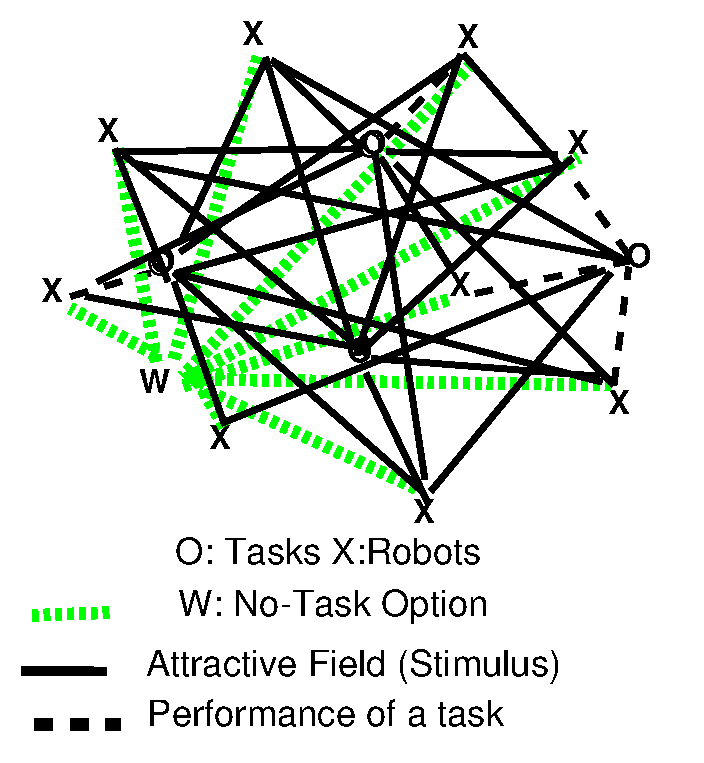
\includegraphics[height=0.5\textwidth, angle=0]{./AFM-Diag3.eps}
%figure caption is below the figur
\caption{\small Attractive Filed Model (AFM)}
\label{fig:afm} 
\end{figure}
%%
AFM is presented graphically in Fig. \ref{fig:afm}.  The elements depicted are:
\begin{enumerate}
\item Source nodes (o) are tasks to be allocated to agents
\item Agent nodes (x) e.g., ants, humans, or robots
\item Black solid edges represent the attractive fields and correspond to an agent's perceived stimuli from each task.
\item Green edges represent the attractive field of the ever present no-task option, represented as a particular task (w).
\item The black dashed edges are not actual edges, but represent how each agent is allocated to a single task at any given point in time.
\end{enumerate}

The edges of the AFM network are weighted and the value of this weight describes the strength of the stimulus as perceived by the agent.  In a spatial representation of the model, the strength of the field depends on the physical distance of the agent to the source.  In information-based models, the distance can represent an agent's level of understanding of that task.  The strength of a field is increased through the sensitisation of the agent through experience with performing the task.  This elements is not depicted explicitly in Figure~\ref{fig:afm} but is represented in the weights of the edges.  In Figure~\ref{fig:afm}, the nodes have arbitrary positions.  Even though the distance is physical in this case, it need not be.  When the model is applied to other domains, the distance can represent the accessibility of information or the time the information takes to reach the agent. 
In summary, from the above diagram of the network, we can see that each of the agents is connected to each of the tasks. This means that even if an agent is currently involved in a task, the probability that it stops doing it in order to pursue a different task, or to random walk, is always non-zero.

AFM assumed a repeated task selection by individual agents.  The probability of an agent choosing to perform a task is proportional to the strength of the task's attractive field, as given by Equation~\ref{eqn:afm3}.
\begin{equation}
P_{j}^{i} = \frac{S_{j}^{i}}{\sum_{j=0}^{J} S_{j}^{i}} \hspace*{0.25cm}where,\hspace*{0.25cm}S^{i}_{0} = S^{i}_{RW}   
\label{eqn:afm3}
\end{equation}
Equation~\ref{eqn:afm3} states that the probability of an agent, $i$, selecting a task, $j$, is proportional to the stimulus, $ S^i_j$, perceived from that task, with the sum of all the task stimuli normalised to $1$.

The strength of an attractive field varies according to how sensitive the agent is to that task, $k_{j}^{i}$, the distance between the task and the agent, $d_{ij}$, and the {\em urgency}, $\phi _{j}$ of the task.  In order to give a clear edge to each field, its value is modulated by the hyperbolic tangent function, $tanh$.  Equation~\ref{eqn:afm1} formalises this part of AFM.
%% S
\begin{equation}
S_{j}^{i} = tanh\{\frac{k_{j}^{i}}{d_{ij}+\delta } \phi _{j}\}
\label{eqn:afm1}
\end{equation}
Eqation~\ref{eqn:afm1}, used small constant $\delta$, called {\em delta distance}, to avoid division by zero, in the case when a robot has reached to a task.

Equation~\ref{eqn:afm2} shows how AFM handles the the no-task, or random walk, option.  The strength of the stimuli of the random walk task depends on the strengths of the fields of real tasks.  In particular, when the other tasks have a low overall level of sensitisation, i.e., relatively weak fields, the strength of the random walk field is relatively high.  On the other hand, when the agent is highly sensitised, the strength of the random walk field becomes relatively low.  We use $J$ to denote the number of real tasks.  AFM effectively considers random walking as an ever present additional task.  Thus the total number of tasks becomes $J+1$. %--P(Task)
\begin{equation}
S^{i}_{RW} = tanh \left \{ 1 -  \frac{ \sum_{j=1}^{J} S^{i}_{j}}{J + 1} \right \}
\label{eqn:afm2}
\end{equation}
%-- P(RW)

A task $j$ has an associated urgency $\phi_j$ indicating its relative importance over time.  If an agent attends a task $j$ in time step $t$, the value of $\phi_j$ will decrease by an amount $\delta_{\phi_{DEC}}$ in the time-step $t+1$.  On the other hand, if a task has not been served by any of the agents in time-step $t$, $\phi_j$ will increase by a different amount, $\delta_{\phi_{INC}}$ in time-step $t+1$.  This behaviour is formalised in Equations~\ref{eqn:delta-phi1} and~\ref{eqn:delta-phi2} respectively.
%%
\begin{equation}
 If\hspace*{0.15cm}the \hspace*{0.15cm}task\hspace*{0.15cm}is\hspace*{0.15cm}being\hspace*{0.15cm}done:\hspace*{0.15cm}  \phi_{j,t+1} \rightarrow \phi_{j,t} \hspace*{0.15cm} - n\hspace*{0.10cm}\delta_{\phi_{DEC}}
\label{eqn:delta-phi2}
\end{equation}
%%
\begin{equation}
 If\hspace*{0.15cm}the\hspace*{0.15cm} task\hspace*{0.15cm}is\hspace*{0.15cm}not\hspace*{0.15cm}being\hspace*{0.15cm} done:\hspace*{0.15cm} \phi_{j,t+1} \rightarrow \phi_{j,t} \hspace*{0.15cm} + \delta_{\phi_{INC}}
\label{eqn:delta-phi1}
\end{equation}
%%
Equation~\ref{eqn:delta-phi1} refers to a case where no agent attends to task $j$ and Equation~\ref{eqn:delta-phi2} to the case where $n$ agens are concurrently performing task $j$.

In order to complete a task, an agent needs to be within a fixed distance of that task.  When an agent performs a task, it learns about it and this will increases the probability of that agent for selecting that task in the future.  This is done by increasing its sensitization to the task by a fixed amount, $k_{INC}$. The variable affinity of an agent, $i$, to a task, $j$, is called its {\em sensitization} to that task and is denoted $k^{i}_{j}$.  If an agent, $i$, does not do a task $j$, $k^i_j$ is decreased by a different fixed amount, $k_{DEC}$.  This behaviour is formalised in Equations~\ref{eqn:k-inc} and~\ref{eqn:k-dec} respectively.
\begin{equation}
 If\hspace*{0.15cm}task\hspace*{0.15cm}is\hspace*{0.15cm}done:\hspace*{0.15cm}  k^i_j \rightarrow   k^i_j \hspace*{0.15cm} + \hspace*{0.15cm} k_{INC}
\label{eqn:k-inc}
\end{equation}
\begin{equation}
 If\hspace*{0.15cm}task\hspace*{0.15cm}is\hspace*{0.15cm}not\hspace*{0.15cm}done:\hspace*{0.15cm}  k^i_j \rightarrow   k^i_j \hspace*{0.15cm} - \hspace*{0.15cm} k_{DEC}
\label{eqn:k-dec}
\end{equation}
%%
The interpretation of AFM in a multi-robot system follows the above mentioned generic interpretation. Each robot can be modelled as an agent and each task can be modelled as a spatial location. Depending on a specific task performance, sensitization levels of robots for that task can be increased or decreased. Robots can have multiple options to select a task from a set of available tasks. If there is only a global task, e.g. in case of foraging task, random walking can be used as a no-task option. Thus using this abstract approach, we can effectively model the MRTA issue of a global task as well as multiple concurrent tasks in a multi-tasking environment. The distance between a task and a robot is simply the physical distance and the sensitivities are recorded as specific values on each robot. The urgency values of the tasks are calculated based on the number of robots attending each task and the updated urgency values are communicated to the robots.

The sensing of the distance between the tasks and robots as well as the communication of urgency values are non-trivial in a robotic system.  Both the sensing and communication can be done either locally by the individual robots or centrally, through an overhead camera and a global communication network.
This article focuses on investigating the role of latter strategy on the performance of self-organized MRTA.
%--------------------------------------
\subsection{Task-Allocation in a Manufacturing Shop-Floor Scenario}
\label{sec:mrta}
%%
\begin{figure}[htp]
\centering
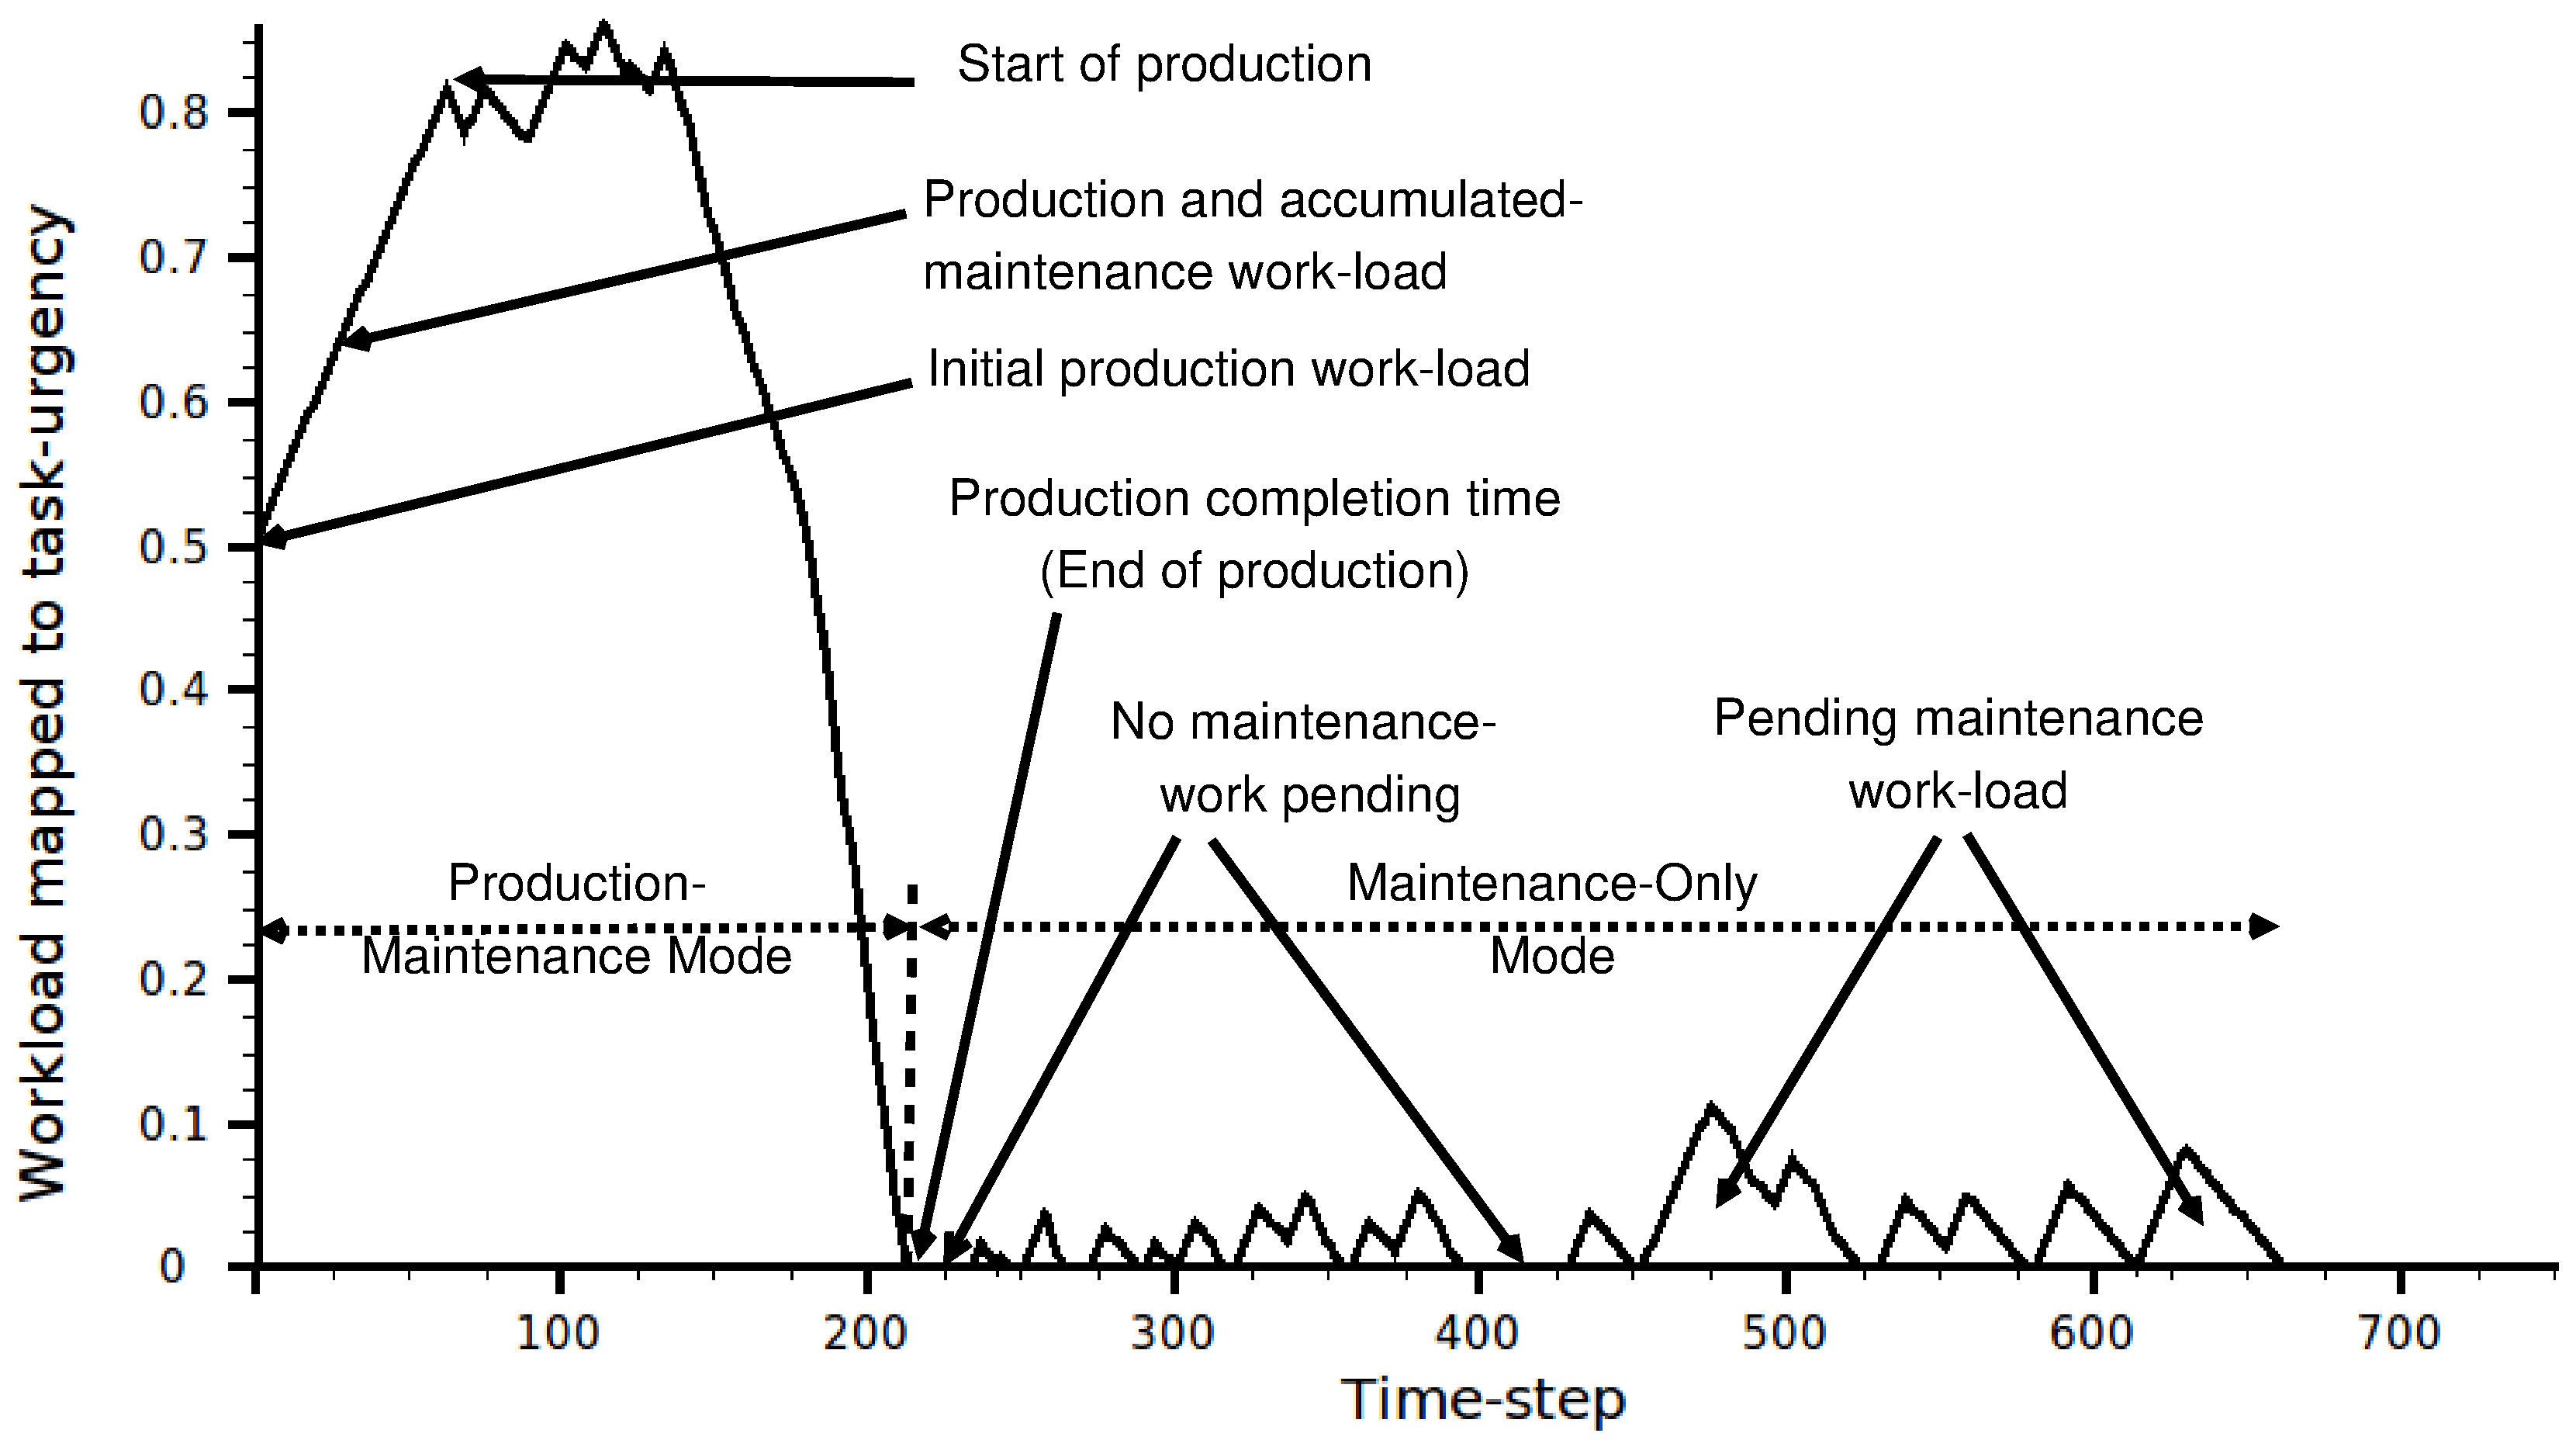
\includegraphics[width=0.8\textwidth, angle=0]
{./VSP.eps}
%figure caption is below the figure
\caption{\small Virtual Shop-floor production and maintenance cycle}
\label{fig:vsp}  % Give a unique label
\end{figure}
%%
One of the major issues that need to be addressed before applying AFM in real-world problem is how to map various properties of AFM to that of the given problem. Here we have designed a manufacturing shop-floor scenario that demonstrates this. By extending our interpretation of AFM in multi-robot system, in our  manufacturing shop-floor  scenario we translate the task-requirements and robot capabilities into task-urgency values. In this scenario, each task represents a manufacturing machine. These machines are capable of producing goods from raw materials, but they also require constant maintenance works for stable operations. Let $W_{j}$ be a finite number of material parts that can be loaded into a machine $j$ in the beginning of its production process and in each time-step, $\omega_{j}$ units of material parts can be processed  ($\omega_{j} \ll W_{j} $). So let $\Omega_{j}^{p}$ be the initial production workload of $j$ which is simply: $W_{j} / \omega_{j}$ unit. We assume that all machines are identical. In each time step, each machine always requires a minimum threshold number of robots, called hereafter as {\em minimum robots per machine ($\mu$)}, to meet its constant maintenance work-load, $\Omega_{j}^{m}$ unit. However, if $\mu$ or more robots are present in a machine for production purpose, we assume that, no extra robot is required to do its maintenance work separately. These robots, along with their production jobs, can do necessary maintenance works concurrently. For the sake of simplicity, in this paper we consider $\mu$ = 1.

The above production and maintenance work-loads and task performance of robots are represented on a task-urgency unit scale.  The manufacturing operation is divided into two subsequent stages: i) {\em production and maintenance mode (PMM)} or simply called {\em production cycle}, and ii) {\em maintenance only mode (MOM)} or simply called {\em maintenance cycle}. Initially a machine starts working in production cycle and does production and maintenance works concurrently. When there is no production work left, it then enters into maintenance cycle. Fig. \ref{fig:vsp} illustrates this for a single machine.

Under both modes, $\alpha_{j}$ is the amount of workload occurs in a unit time-step if no robot serves a task and it corresponds to a fixed task-urgency $\Delta \phi_{INC}$.  Simultaneously, for each time-step, a robot, $i$, can decrease the constant workload $\beta_{i}$ by doing some maintenance work along with doing any available production work.  This corresponds to a negative task urgency: $- \Delta \phi_{DEC}$. 
So, at the beginning of production process, task-urgency, occurred in a machine due to its production work-loads, can be encoded by Eq. \ref{eqn:task-urgency-prod-init}.
\begin{equation}
%\small
\Phi_{j, INIT}^{PMM} = \Omega_{j}^{p} \times \Delta \phi_{INC} + \phi_{j}^{m0}
\label{eqn:task-urgency-prod-init}
\end{equation}
where $\phi_{j}^{m0}$ represents the task-urgency due to an initial maintenance work-load of $j$.
Now if no robot attends to serve a machine, each time-step a constant maintenance workload of $\alpha_{j}^{m}$ will be added to $j$ and that will increase its task-urgency by $\Delta \phi_{INC}$. So, if k time steps passes without any production work being done, task urgency at $k^{th}$ time-step will follow Eq. \ref{eqn:task-urgency-prod-case1}.
\begin{equation}
\Phi_{j, k}^{PMM} =\Phi_{j, INIT}^{PMM} + k \times \Delta \phi_{INC}
\label{eqn:task-urgency-prod-case1}
\end{equation}
However, if a robot attends to a machine and does some production works from it, there would be no extra maintenance work as we assumed that $\mu$ = 1. Rather, the task-urgency on this machine will decrease by $\Delta \phi_{DEC}$ amount. If $\nu_{k}$ robots work on a machine simultaneously at time-step $k$, this decrease will be: $\nu_{k} \times \Delta \phi_{DEC}$. So in such cases, task-urgency in $(k+1)^{th}$ time-step can be represented by:
\begin{equation}
\Phi_{j, k+1}^{PMM} = \Phi_{j, k}^{PMM} - \nu_{k} \times \Delta \phi_{DEC}
\label{eqn:task-urgency-prod-case2}
\end{equation}
At a particular machine $j$, once $\Phi_{j, k}^{PMM}$ reaches to zero, we can say that there is no more production work left and this time-step $k$ can give us the {\em production comparison time} of $j$, $T_{j}^{PMM}$. Average production time-steps of a shop-floor with M machines can be calculated by the following simple equation.
\begin{equation}
T_{avg}^{PMM} = \frac{1}{M} \sum_{j=0}^{M} T_{j}^{PMM} 
\label{eqn:avg-pmm}
\end{equation}
$T_{avg}^{PMM}$ can be compared with the minimum number of time-steps necessary to finish production works, $T_{min}^{PMM}$. This can only happen in an ideal case where all robots work for production without any random walking or failure. We can get $T_{min}^{PMM}$ from the total amount of work load and maximum possible inputs from all robots. If there are M machines and N robots, each machine has $\Phi_{INIT}^{PMM}$ task-urgency, and each time-step robots can decrease N $\times$ $\Delta \phi_{DEC}$ task-urgencies, then the theoretical $T_{min}^{PMM}$ can be found from the following Eq. \ref{eqn:min-pmm}.
%
\begin{multicols}{2}
\small
\begin{equation}
T_{min}^{PMM} = \frac{M \times \Phi_{INIT}^{PMM}}{N \times \Delta \phi_{DEC}} 
\label{eqn:min-pmm}
\end{equation}
\vspace*{0.2cm}
\begin{equation}
\zeta_{avg}^{PMM} = \frac{T_{avg}^{PMM} - T_{min}^{PMM}}{T_{min}^{PMM}} 
\label{eqn:appd}
\end{equation}
\end{multicols}
Thus we can define $\zeta_{avg}^{PMM}$, {\em average production completion delay} (APCD) by following Eq. \ref{eqn:appd}.
%%
When a machine enters into maintenance cycle, only $\mu$ robots are required to do its maintenance works in each time step. So, in such cases, if no robot serves a machine, the growth of task-urgency will follow Eq. \ref{eqn:task-urgency-prod-case1}. However, if $\nu_{k}$ robots are serving this machine at a particular time-step $k^{th}$ , task-urgency at $(k+1)^{th}$ time-step can be represented by:
\begin{equation}
\Phi_{j, k+1}^{MOM} = \Phi_{j, k}^{MOM}- (\nu_{k} - \mu) \times \Delta \phi_{DEC}
\label{eqn:task-urgency-maint-case}
\end{equation}
By considering $\mu = 1$, Eq. \ref{eqn:task-urgency-maint-case} will reduces to Eq. \ref{eqn:task-urgency-prod-case2}. Here, $\Phi_{j, k+1}^{MOM}$ will correspond to the {\em pending maintenance work-load (PMW)} of a particular machine at a given time. This happens due to the random task switching of robots with a no-task option (random-walking). Interestingly PMW will indicate the robustness of this system since higher PMW value will indicate the delay in attending maintenance works by robots. This also means how much time a machine is left unattended by all robots. We can find the average PMW (APMW) per time-step for an individual  machine, $\chi_{j}^{MOM}$ (Eq. \ref{eqn:sigle-pmw}) and average PMW per machine per time-step, $\chi_{avg}^{MOM}$ (Eq. \ref{eqn:avg-pmw}).
\begin{multicols}{2}
\small
\begin{equation}
\chi_{j}^{MOM}= \frac{1}{K} \sum_{k=1}^{K} \Phi_{j, k}^{MOM}
\label{eqn:sigle-pmw}
\end{equation}
\vspace*{0.2cm}
\begin{equation}
\chi_{avg}^{MOM}= \frac{1}{M} \sum_{j=1}^{M} {\chi_{j}^{MOM}}
\label{eqn:avg-pmw}
\end{equation}
\end{multicols}
%%=========================================================
\section{Centralized Communication Scheme}
\label{sec:comm}
\begin{figure}
\centering
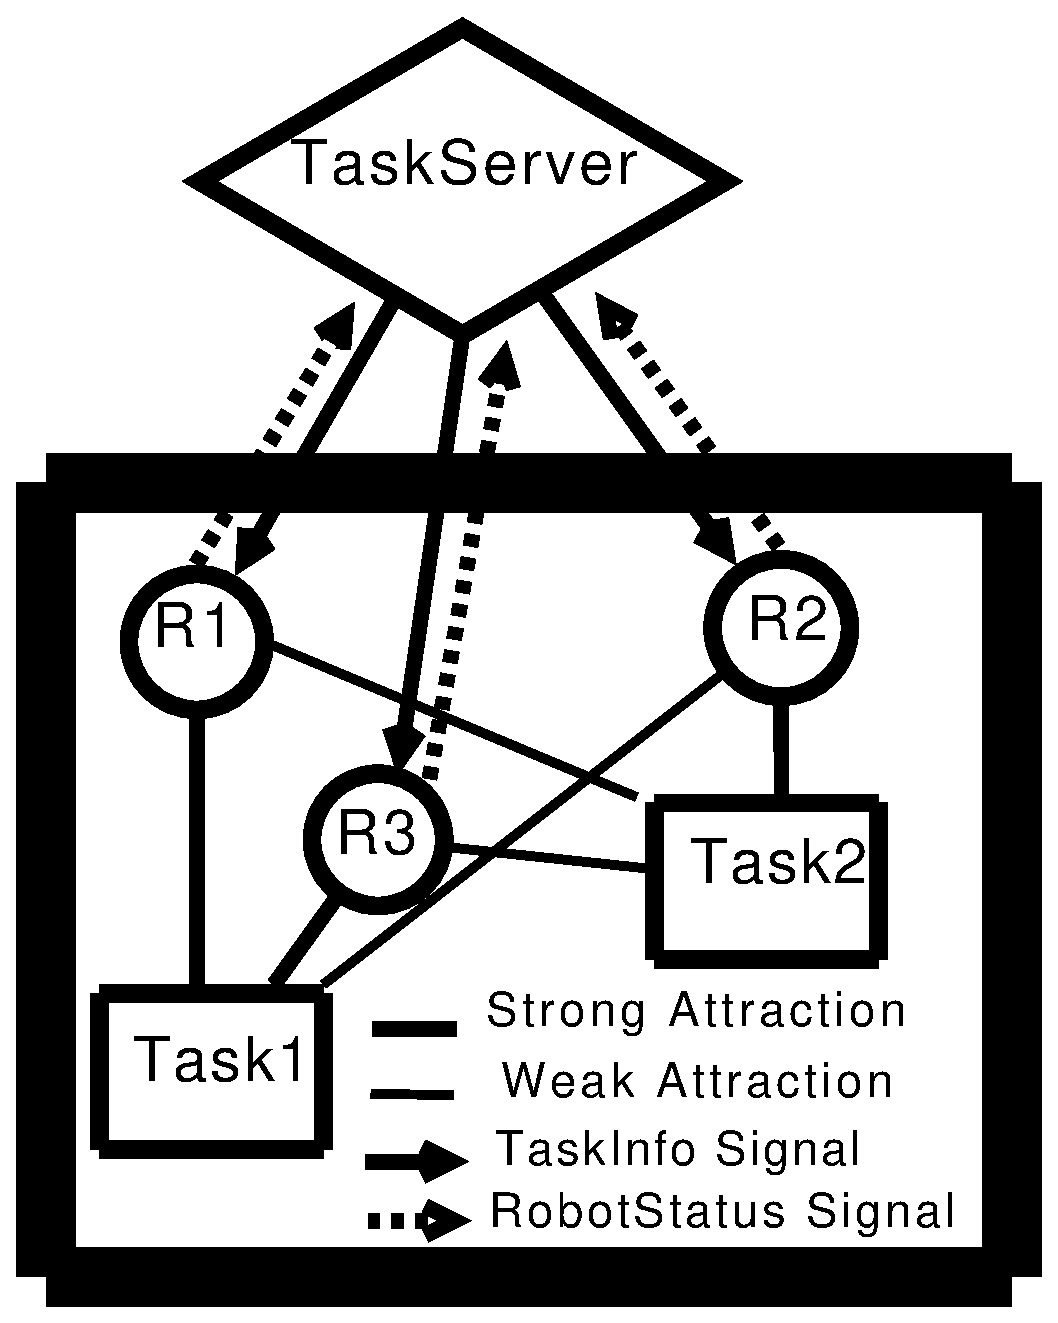
\includegraphics[height=0.5\textwidth, angle=0]{./CentralizedComm.eps}
\caption{\small A centralized communication scheme} % for implementing AFM}
\label{fig:ccm} % Give a unique label
\end{figure}
%%
The continuous flow of information in AFM can be realized using any suitable communication model. The abstract view of our centralized point-to-point communication scheme is outlined in Fig. \ref{fig:ccm}. In this model bi-directional signal-based exchange of communication messages are shown between the centralized entity, i.e. a task server, and robot-controller units, e.g. R1, R2, etc. The main role of task server is to send up-to-date task-information to robot-controllers. 

Our communication scheme can be characterized in terms of three fundamental issues of communication: i) message content, ii) communication frequency and iii) target message recipients \citep{Gerkey+2001}. AFM suggests the communication of task-urgencies among robots. This communication helps the robots to gain information about their tasks and environment. However in this communication scheme robots do not perform any peer-to-peer communication among themselves.  In order to run the task-allocation algorithm robot-controllers need the distance to task information. Since our robots have no suitable sensor to estimate this directly, the task position information is included in the message. Our centralized communication scheme is open to include any further information, such as time-stamp. Thus our centralized point-to-point communication scheme spread the attractive fields of all tasks globally to all robots.
%%%%%%%%%%%%%%%%%%%%%%%%%%%%%%%%%%%%%%%%%%%%%%%%%%%%%%%%%%%%%%%%%%%%%%%%%%%%
\section{Experiments}
\label{sec:expt}
Since AFM is an abstract framework for task-allocation our experiments have been designed to test whether AFM can be instantiated successfully as a practical MRTA platform by showing necessary properties of division of labour, such task specialization, dynamic task-switching or plasticity,  task performance variation over time and so forth. Particularly, in this paper we present our experiments that validate AFM relying upon a centralized point-to-point communication scheme that generates the continuous flow of information. Thus a set of observables has been chosen carefully to observe the convergence of  task-allocation among the robots and, at the same time, to find out the effectiveness of our communication scheme in producing those task-allocation solutions. Here we have described the design of the observables and parameters of our experiments within the context of our manufacturing shop-floor scenario.  We have briefly included the implementation platform. The details of our multi-robot control architecture has been discussed in \cite{Sarker2010control}.
\subsection{Observables}
In our experiments the following characteristics have been observed within the context of self-organized MRTA.

\textbf{Plasticity:} %As we have discussed in Sec. \ref{bg:def:MRTA},  
Self-organized MRTA is often characterised by the plasticity and task specialization, in both macroscopic and microscopic levels. Within our manufacturing shop-floor context, plasticity refers to the collective ability of the robots to switch from doing no-task option (random-walking) to doing a task (or vice-versa) depending on the work-load present in the system. Here we expect to see that most of the robots would be able to engage in tasks when there would be high workloads (or task-urgencies) during the production cycle of our manufacturing shop-floor scenario. Similarity, when there would be low workload in case of the maintenance cycle of our manufacturing shop-floor scenario, only a few robots would do the task, rest of them would either be idle (not doing any task) or perform a random-walk.  The changes of task-urgencies and the ratio of robots engaged in tasks can be good metrics to observe plasticity in MRTA.

\textbf{Task-specialization:} Self-organized MRTA is generally accompanied with task specializations of agents. That means that few robots will be more active than others. From the interpretation of AFM, we can see that after doing a task a few times, a robot will soon be sensitized to it. Therefore, from the raw log of task-sensitization of robots, we can be able to find the pattern of task-sensitization of robots per task basis.

\textbf{Quality of task-performance:} The quality of MRTA can be measured from the production delay value. It first calculates the ideal minimum production time and then finds the delay in production process from the actual production completion data. Thus this will indicate how much more time is  spent in the production process due to the self-regulation of robots in this distributed task-allocation scheme.  In order to calculate production delay, we can find the production completion time for each task from the raw log of task-urgency and make an average from them.

\textbf{Robustness:} In order to see if our system can respond to the gradually increasing workloads,  we can measure pending maintenance workload (i.e. APMW) within the context of our manufacturing shop-floor scenario. This pending maintenance workload indicates how much a machine is left unattended by all the robots on an average. This measures the robustness of our system where robots often leave a task in favour of another one. When a task is not being served by any robot for some time we would be able to see that its urgency would rise and robots would respond to this dynamic demand. For measuring pending maintenance workload we need only the task-urgency data.

\textbf{Flexibility:} From the design of AFM, we know that robots that are not doing a task will be de-sensitized to it or forget that task. So at an overall low work-load (or task urgency), less robots will do the tasks and hence less robots will have the opportunity to learn tasks. From the shop-floor work-load data, we can confirm the presence of flexibility in MRTA.

\textbf{Energy-efficiency:} In order to characterize the energy-efficiency in MRTA we can log the pose data of each robot that can give us the total translations occurred by all robots in our experiments. This can give us a rough indication of energy-usage by our robots. 

\textbf{Information flow:} Since AFM requires a system-wide continuous flow of information, we can measure the communication load to bench-mark our implementation of communication system. This bench-mark data can be used to compare among various communication strategies. Here we can measure  how much task-related information, i.e. task-urgency, location etc. are sent to the robots at each time step. This  amount of information or communication load can be constant or variable depending on the design of the communication system.

\textbf{Scalability:} In order to see the effects of scaling on MRTA, we have designed two group of experiments. Series A corresponds to a small group where we have used 8 robots, 2 tasks under an arena of 2m by 1m. We have doubled these numbers in Series B (Table \ref{table:params}). This proportional design can give us a valuable insight about the effects of scaling on self-organized MRTA. 

Thus, in order to observe the above properties of self-organized MRTA, we have designed our experiments to record the following  observables in each time-step.
\begin{enumerate}
\item Task-urgency of each task ($\phi$).
\item Number of robots engaged in each task.
\item Task-sensitizations ($k$) of robots.
\item Pose data of robots.
\item Communication of task-information message among TPS and RCCs.  
\end{enumerate}
%%
\begin{table}
\caption{Experimental parameters of Series A \& B experiments}
\label{table:params}
\begin{center}
\begin{tabular}{|p{2in}|c|}
\hline Parameter & Series A $\mid$ Series B\\
\hline Total number of robots ($N$) & \hspace*{0.1cm} 8 $\mid$ 16\\
\hline Total number of tasks ($M$) & 2 $\mid$ 4\\
\hline Experiment area ($A$) & 2 $m^2$ $\mid$  4 $m^2$\\
\hline Initial production work load/machine ($\Omega_{j}^{p}$) & 100 unit \\
\hline Task urgency increase rate ($\Delta\phi_{INC}$) & 0.005\\
\hline Task urgency decrease rate ($\Delta\phi_{DEC}$) & 0.0025\\
\hline Initial sensitization ($K_{INIT}$) & 0.1\\
\hline Sensitization increase rate ($\Delta k_{INC}$) & 0.03\\
\hline Sensitization decrease rate ($\Delta k_{DEC}$) & 0.01\\
\hline
\end{tabular}
\end{center}
\end{table}
%%
%------------------------------------------------------------
\subsection{Parameters}
Table \ref{table:params} lists a set of essential parameters of our experiments. We intend to have a set-up that is relatively complex, i.e., with a high number of robots and tasks in a large area. The diameter of the marker of our e-puck robot is 0.08m. So, if we put 4 robots in an area of one square meter, this will give us a robot-occupied-space to free-space ratio of about 1:49 per square meter. This ratio is reasonable in order to allow the robots to move at a speed of 5 cm/sec without causing much interference to each other. 

The initial values of task urgencies correspond to 100 units of production work-load without any maintenance work-load as outlined in Eq. \ref{eqn:task-urgency-prod-init}. We choose a limit of 0 and 1, where 0 means no urgency and 1 means maximum urgency. Same rule applies to sensitisation, where 0 means no sensitisation and 1 means maximum sensitisation. This also implies that if sensitization is 0, task has been forgotten completely. On the other hand, if sensitization is 1, the task has been learnt completely. We choose an initial sensitization value of 0.1 for all tasks. The following relationships are maintained for selecting task-urgency and sensitization parameters.
\begin{equation}
\Delta\phi_{INC} = \frac{\Delta\phi_{DEC} \times N}{2 \times M}
\label{eqn:task-urgency}
\end{equation}
%
\begin{equation}
\Delta k_{DEC} = \frac{\Delta k_{INC}} {M - 1} 
\label{eqn:sensitization}
\end{equation}
%
Eq. \ref{eqn:task-urgency} establishes the fact that task urgency will increase at a higher rate than that of its decrease. As we do not like to keep a task left unattended for a long time we choose a higher rate of increase of task urgency. This difference is set on the basis of our assumption that robots are incapable of doing a task by itself alone. So more robots are attracted towards a task.

Eq. \ref{eqn:sensitization} suggests that the learning will happen much faster than the forgetting. The difference in these two rates is based on the fact that faster leaning gives a robot more chances to select a task in next time-step and thus it becomes quickly specialized on it.
%%%%%%%%%%%%%%%%%%%%%%%%%%%%%%%%%%%%%%%%%%%%%%%%%%%% 
\subsection{Implementation}
\label{sec:impl}
\begin{figure}
\centering
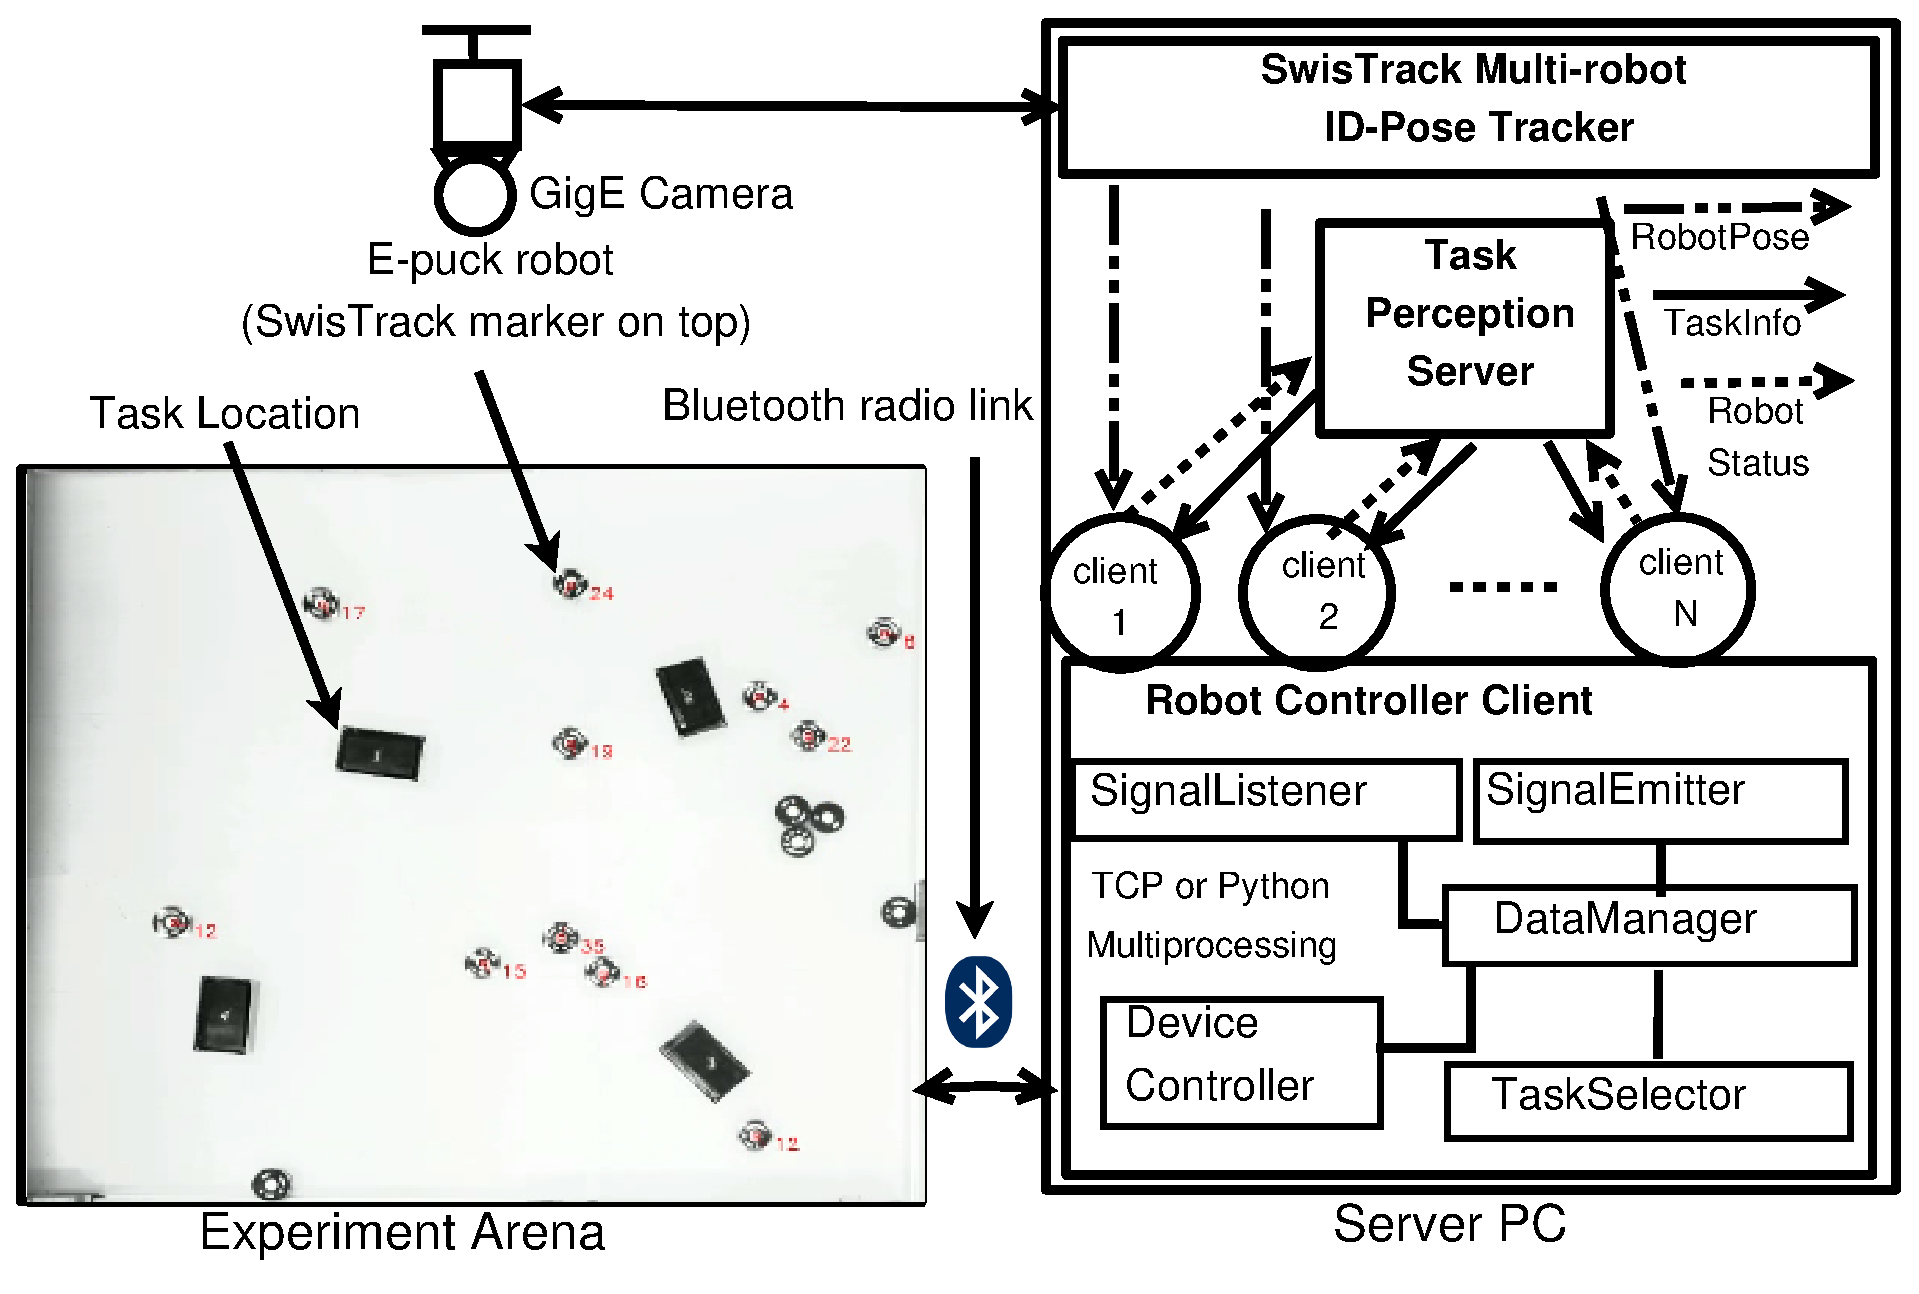
\includegraphics[width=0.9\textwidth, angle=0]
{./RIL-Expt-Setup1.eps}
%figure caption is below the figure
\caption{\small Hardware and software setup}
\label{fig:setup} % Give a unique label
\end{figure}
As shown in Fig. \ref{fig:setup}, three major software systems have been implemented for validating AFM: i) \textit{TaskPerceptionServer} (TPS), ii) \textit{RobotController Client} (RCC) and iii) SwisTrack multi-robot tracker \citep{Lochmatter+2008}. The centralized TPS is responsible for disseminating task information to RCCs. TPS delivers this information by emitting \textit{TaskInfo} signals periodically. This task-information mainly contains the relevant task information which is used by the our high-level robot-controller RCCs for running their task-allocation algorithm. TPS has another interface for catching feedback signals from RCCs. The \textit{RobotStatus} signal can be used to inform TPS of a robot's current task ID, its device status etc. Upon  receiving this information, TPS updates relevant part of task information such as, task-urgency.  SwisTrack  tracks all e-puck\footnote{www.e-puck.org} robots in real-time using a 16-megapixel overhead Prosilica GigE 4900C\footnote{www.prosilica.com}  camera. This set-up produces the position, orientation and ID of all  robots by processing the image frames at 1.5 FPS.  

For inter-process communication among all the above software components, we have used D-Bus technology \citep{Pennington+2010}. An inter-process communication module for SwisTrack has been developed that can broadcast id and pose of all robots in real-time over a common D-Bus interface. RCCs are developed in Python with its state of the art \textit{Multiprocessing}\footnote{http://docs.python.org/library/multiprocessing.html} module. This python module simplifies the need for  sharing data and performing synchronization among different sub-processes. As shown in Fig. \ref{fig:setup}, the software system of a RCC consists of four sub-processes. {\em SignalListener} and {\em SignalEmitter}, interface with SwisTrack's D-Bus communication module and TPS. {\em TaskSelector} implements AFM algorithms for task selection. {\em DeviceController} physically drives a robot towards a target task's boundary. Bluetooth radio link is used as a communication medium between a RCC and a corresponding e-puck robot. The detail design and implementation of our of D-Bus communication scheme can be found in \cite{Sarker2010control}. 
%================================================================= 
\section{Results \& Discussions}
\label{sec:res}
In this section we present and discuss our experimental results. Each experiment, series A and series B consisted of five separate trials the reported results are the trial averages.  Each trial lasted 40 minutes.
%%-------------------------------------------------
\subsection{Results}
\subsubsection{Shop-floor work-load history}
In our experiments we have defined shop-floor work-load in terms of task urgencies. For example, Eq. \ref{eqn:task-urgency-prod-init} shows how we have calculated initial production work-load of our manufacturing shop-floor scenario.  Fig. \ref{fig:raw-urgencies-SA} and Fig. \ref{fig:raw-urgencies-SB}  show the dynamic changes in task-urgencies for the single iteration of Series A and Series B experiments respectively. The fluctuations in these plots are resulted from the different levels of task-performance of our robots.
\begin{figure}
%\begin{minipage}[t]{0.48\linewidth}
\centering
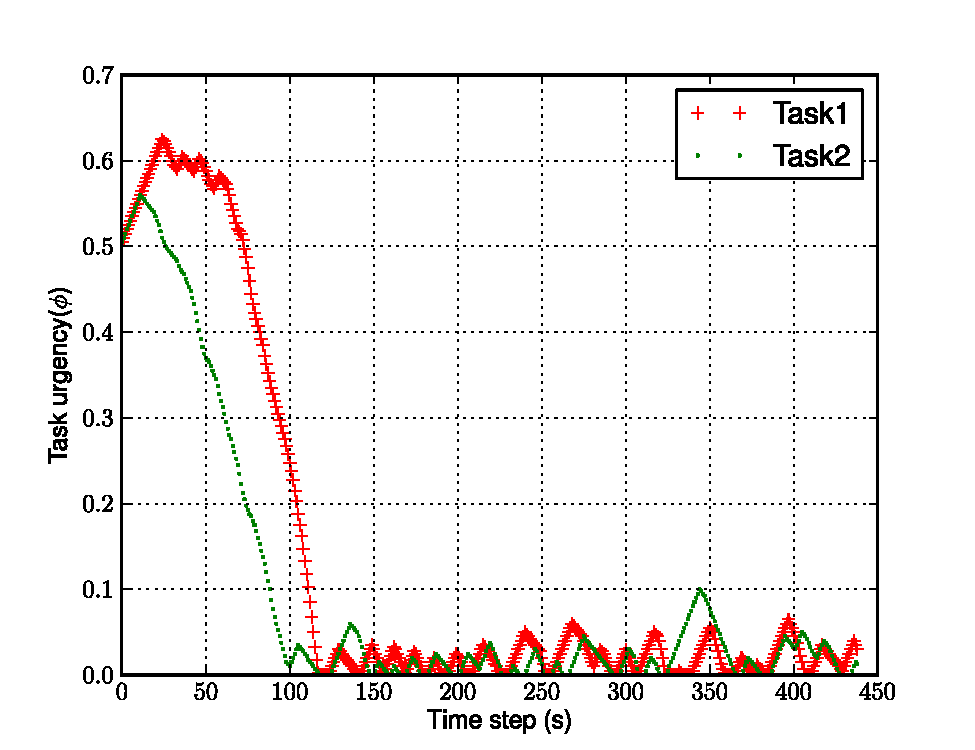
\includegraphics[width=0.7\textwidth, angle=0]
{./PlotUrgencyLog-2010Apr30-095755.eps}
%figure caption is below the figure
\caption{\small Changes in task-urgencies in Series A experiments}
\label{fig:raw-urgencies-SA} 
%\end{minipage}
%\hspace{0.5cm}
%\begin{minipage}[t]{0.48\linewidth}
\centering
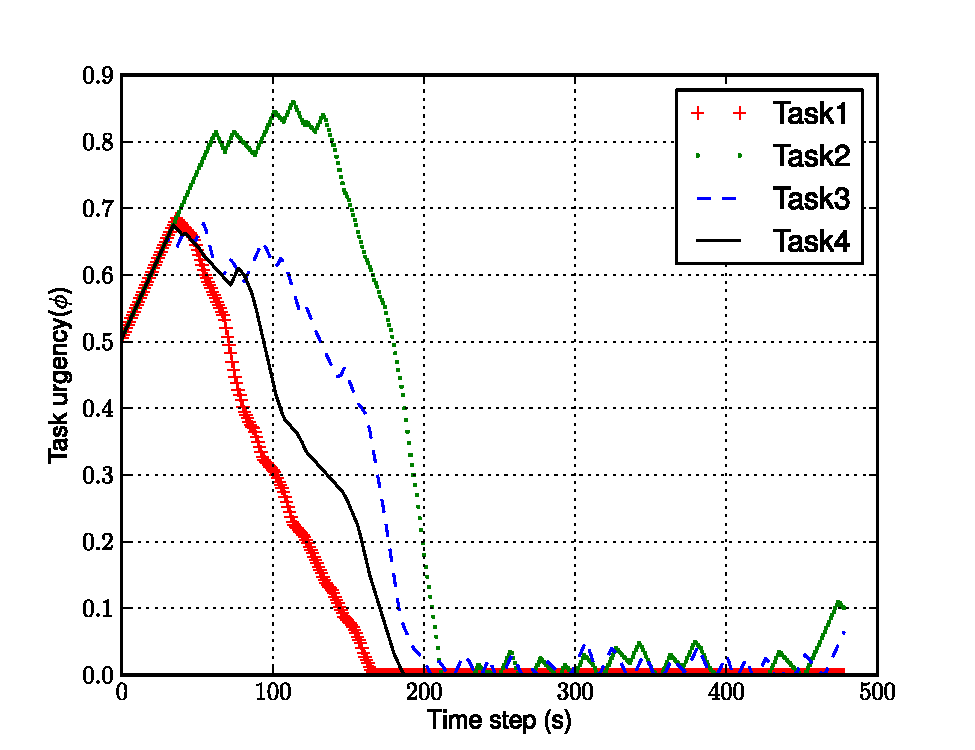
\includegraphics[width=0.7\textwidth, angle=0]{./PlotUrgencyLog-2010May10-115549.eps}
\caption{\small Changes in task-urgencies in Series B experiments} 
\label{fig:raw-urgencies-SB} 
%\end{minipage}
\end{figure}
In order to measure the task-related work-loads on our system we have summed up the changes in all task-urgencies over time. We call this as {\em shop-floor work-load history} and formalized as follows. Let $ \phi_{j, q}$ be the urgency of a task $j$ at $q^{th}$ step and $\phi_{j, q+1}$ be the task urgency of $(q+1)^{th}$ step. We can calculate the sum of changes in urgencies of all $M$ tasks at $(q+1)^{th}$ step:
\begin{equation} 
\Delta \Phi_{j, q+1} = \sum_{j=1}^{M} (\phi_{j, q+1} - \phi_{j, q})
\label{eqn:Delta-Phi}
\end{equation}
From Fig. \ref{fig:urgency-stat-SA} and Fig. \ref{fig:urgency-stat-SB} show the dynamic shop-floor workload for Series A and Series B experiments respectively. From these plots, we can see that initially the sum of changes of task urgencies (shop-floor workload) is going towards negative direction. This implies that tasks are being served by a high number of robots. 
%%
\begin{figure}
%\begin{minipage}[t]{0.48\linewidth}
\centering
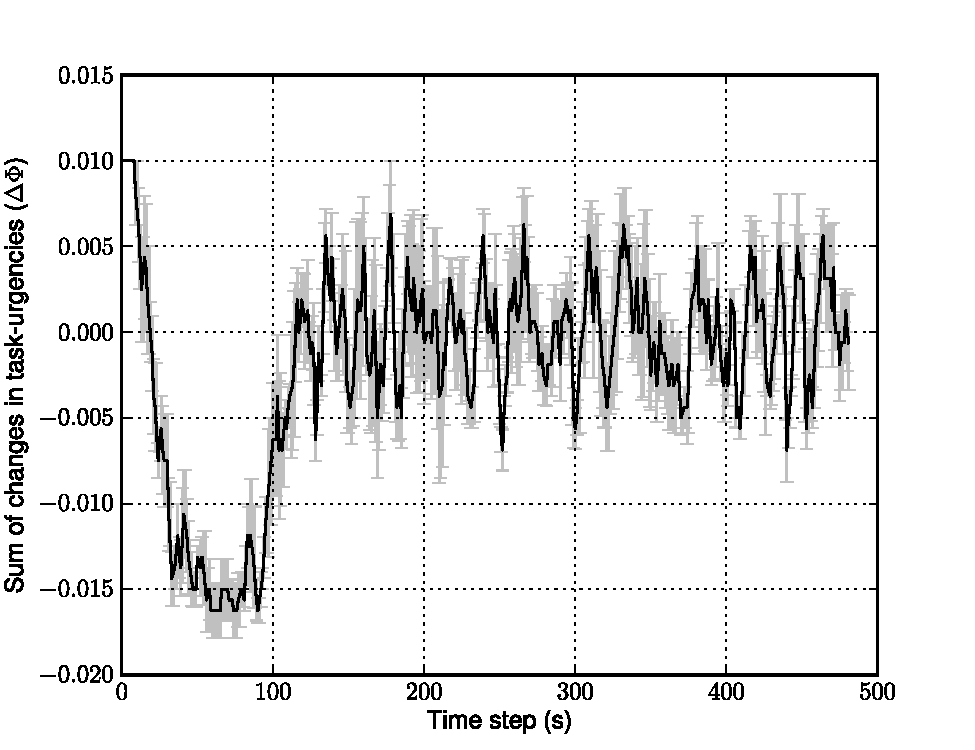
\includegraphics[width=0.7\textwidth, angle=0]
{./8robots2tasks-TaskUrgencyStat.eps}
%figure caption is below the figure
\caption{\small Shop-floor workload change history in Series A} 
\label{fig:urgency-stat-SA} % Give a unique label
%\end{minipage}
%\hspace{0.5cm}
%\begin{minipage}[t]{0.48\linewidth}
\centering
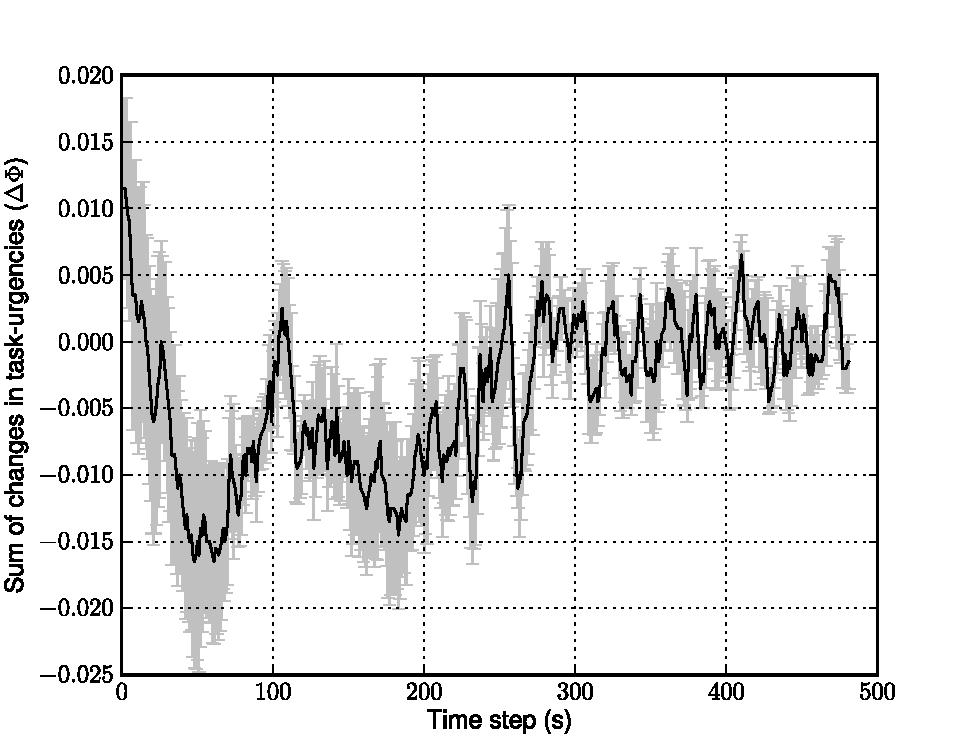
\includegraphics[width=0.7\textwidth, angle=0]{./TaskUrgencyStat.eps}
\caption{\small Shop-floor workload change history in Series B} % measured in terms of task urgencies
\label{fig:urgency-stat-SB} % Give a unique label
%\end{minipage}
\end{figure}
%%
%%----------------------------------------------------------------
\subsubsection{Ratio of active workers}
%%
\begin{figure}
%\begin{minipage}[t]{0.48\linewidth}
\centering
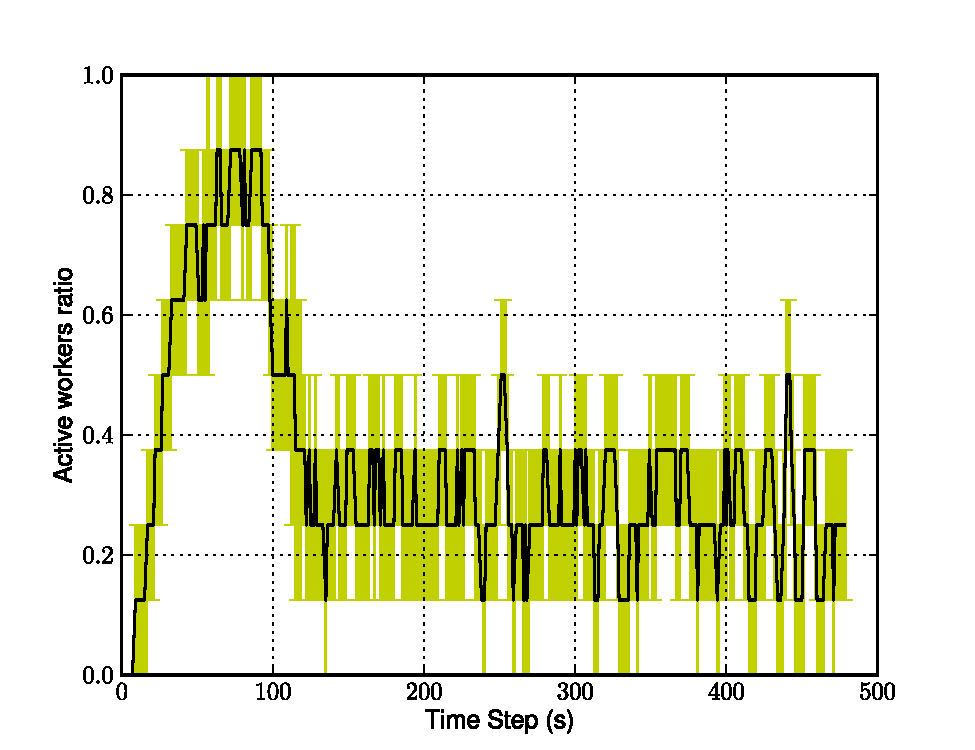
\includegraphics[width=0.7\textwidth, angle=0]
{./Plasticity-8robots2tasks.eps}
%figure caption is below the figure
\caption{\small Self-organized allocation of robots in Series A}
\label{fig:worker-stat-SA}
%\end{minipage}
%
%\hspace{0.5cm}
%\begin{minipage}[t]{0.48\linewidth}
\centering
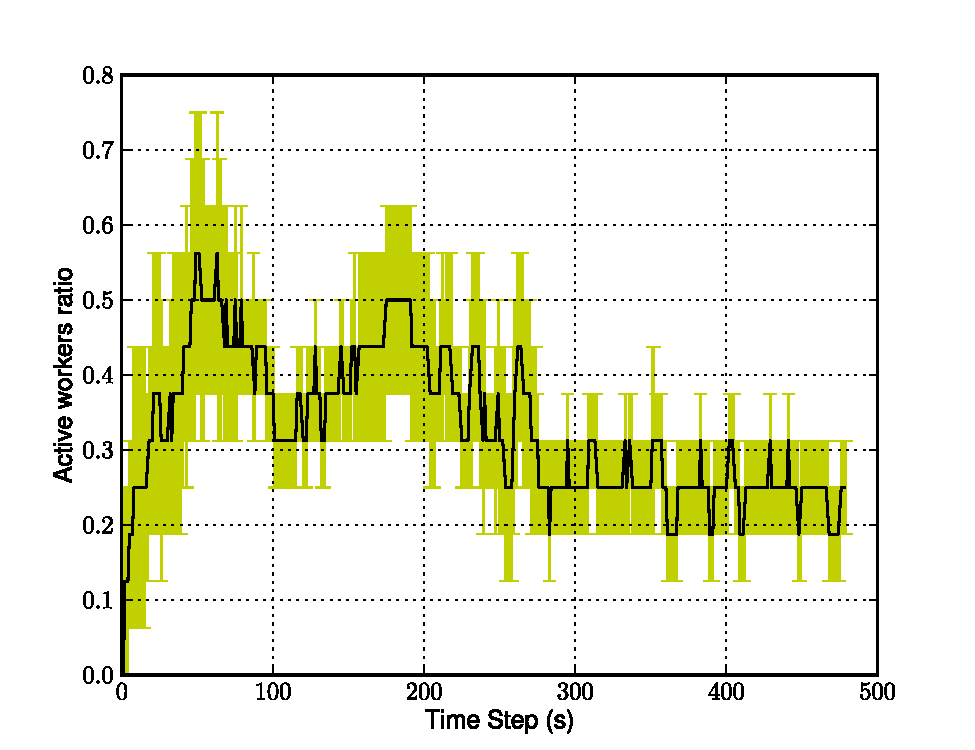
\includegraphics[width=0.7\textwidth, angle=0]{./WorkerRatio.eps}
\caption{\small Self-organized allocation of robots in Series B }
\label{fig:worker-stat-SB} % Give a unique label
%\end{minipage}
\end{figure}
%%
From both Fig. \ref{fig:worker-stat-SA} and Fig. \ref{fig:worker-stat-SB}, we can  see that in production stage, when work-load is high, many robots are active in tasks. Here active workers ratio is the ratio of those robots that work on tasks to the total number of robots ($N$) of a particular experiment.   Here we can see that this ratio varies according to the changes in shop-floor work-load.
%%-------------------------------------------------------------
\subsubsection{Shop-task performance}
In our manufacturing shop-floor scenario, we have calculated the APCD and APMW for both Series A and Series B experiments. For Series A we have got  average production completion time 111 time-steps (555s) where sample size is (5 x 2) = 10 tasks, SD = 10 time-steps (50s). According to Eq. \ref{eqn:min-pmm}, our theoretical minimum production completion time is 50 time-steps (250s) assuming the non-stop task performance of all 8 robots with an initial task urgency of 0.5 for all 2 tasks and task urgency decrease rate $\Delta \Phi_{DEC }$ = 0.0025 per robot per time-step.  Hence, Eq. \ref{eqn:appd} gives us APCD, $\zeta$ = 1.22 which means that in Series A experiments, it took 1.22 times more time (305s) than the estimated minimum production completion time (250s). For Series B, we have got average production completion time 165 time-steps (825s) where sample size is (5 x 4) = 20 tasks, SD = 72 time-steps (360s).  Hence, Eq. \ref{eqn:appd} gives us APCD, $\zeta$ = 2.3.

For APMW, Series A experiments give us an average time length of 369 time-steps (1845s).  In this period we calculated APMW and it is 1 time-step with SD = 1 time-step (5s) and $\Delta \Phi_{INC}$ = 0.005 per task per time-step. This shows a very low APMW ($\chi$ = 0.000235) meaning a very high robustness of the system. For Series B experiments, from the average 315 time-steps (1575s) maintenance activity of our robots per experiment run, we have got APMW, $\chi$ = 0.012756 which corresponds to the pending work of 3 time-steps (15s) where SD = 13 time-steps (65s). This tells us the robust task performance of our robots which can return to an abandoned task within a minute or so.
%%-------------------------------------------------
\subsubsection{Task specializations}
We have measured the task-specialization of the robots based-on their peak value of sensitization. This maximum value represents how long a robot has repeatedly been selecting a particular task. Since tasks are homogeneous we have considered the maximum sensitization value of a robot among all tasks during an experiment run. This value is then averaged for all robots using the following  equation. 
%%
\begin{equation}
K^G_{avg} = \frac{1}{N}\sum_{i=1}^{N} \max_{j=1}^M\left ( k^i_{j, q} \right ) 
\label{eqn:K-G}
\end{equation}
%%
If a robot $r_i$ has the peak sensitization value $k^i_j$ on task $j$ ($j \in M$ tasks)  at $q^{th}$ task-cycle, Eq. \ref{eqn:K-G} calculates the average of the peak task-specialization values of all robots for a certain iteration of our experiments. We have also averaged the task-cycle values ($q$) taken to reach those peak values for all robots using the following equation.
%%
\begin{equation}
Q^G_{avg}= \frac{1}{N}\sum_{i=1}^{N} q^i_{k=k_{max}}
\label{eqn:Q-G}
\end{equation}
In Eq. \ref{eqn:Q-G}, $q^i_{k=k_{max}}$ represents the time-step of robot $r_i$  where its sensitization value $k$ reaches the peak $k_{max}$ as discussed above. By averaging this peak task-cycle values of all robots we can have an overall idea of how many task-execution cycles have been spent to reach the maximum task-specialization value $K^G_{avg}$.
%% S-A
\begin{table}
\centering
\caption{Peak task-sensitization values of robots in a Series A experiment.}
% 30Apr expt.
\begin{tabular}{|c|c|c|c|}
\hline \textbf{Robot ID} & \textbf{Maximum k} & \textbf{At time-step (q)} & \textbf{Task} \\ 
\hline 1 & 0.54 & 64 & Task1\\
\hline 4 & 0.32 & 14 & ,,\\
\hline 5 & 0.27 & 11 & ,,\\
%%
\hline 3 & 0.47 & 63 & Task2\\
\hline 2 & 0.46 & 64 & ,,\\
\hline 6 & 0.20 & 10 & ,,\\
\hline 7 & 0.18 & 4 & ,,\\
\hline 8 & 0.15 & 3 & ,,\\
\hline 
\end{tabular} 
\label{table:K-G-SA}
\end{table}
%% S - B
\begin{table}
\centering
\caption{Peak task-sensitization values of robots in a Series B experiment.}
\begin{tabular}{|c|c|c|c|}
% Apr 18 Feb-3 expt
\hline \textbf{Robot ID} & \textbf{Maximum k} & \textbf{At time-step (q)} & \textbf{Task} \\
\hline 24 & 0.41 & 29 & Task1\\
\hline 13 & 0.31 & 19 & ,,\\
\hline 16 & 0.18 & 4 & ,,\\
%% 
\hline 1 & 0.64 & 66 & Task2\\
\hline 35 & 0.34 & 12 & ,,\\
\hline 5 & 0.28 & 14 & ,,\\
\hline 22 & 0.18 & 20 & ,,\\
\hline 17 & 0.16 & 6 & ,,\\
\hline 3 & 0.14 & 12 & ,,\\
%%
\hline 9 & 0.68 & 66 & Task3\\
\hline 6 & 0.43 & 71 & ,,\\
\hline 15 & 0.19 & 4 & ,,\\
\hline 14 & 0.15 & 4 & ,,\\
\hline 31 & 0.14 & 4 & ,,\\
%%
\hline 19 & 0.22 & 12 & Task4\\
\hline 12 & 0.16 & 10 & ,,\\
\hline 
\end{tabular} 
\label{table:K-G-SB}
\end{table}
Table \ref{table:K-G-SA} and Table \ref{table:K-G-SB} show the peak sensitization values of single iteration of Series A and Series B experiments respectively.  Based on Eq. \ref{eqn:K-G} and Eq. \ref{eqn:Q-G}, we have got the peak task-sensitization $K^G_{avg} 
$ values for Series A: 0.40 (SD=0.08)  and for Series B: 0.30 (SD=0.03), and their respective time-step $Q^G_{avg}$ values: 38 (SD=13) and 18 (SD=5) task-cycles. Here we can see that the robots in Series A had higher chances of task-specialization than that of Series B experiments.
%%--
\begin{figure}
\centering
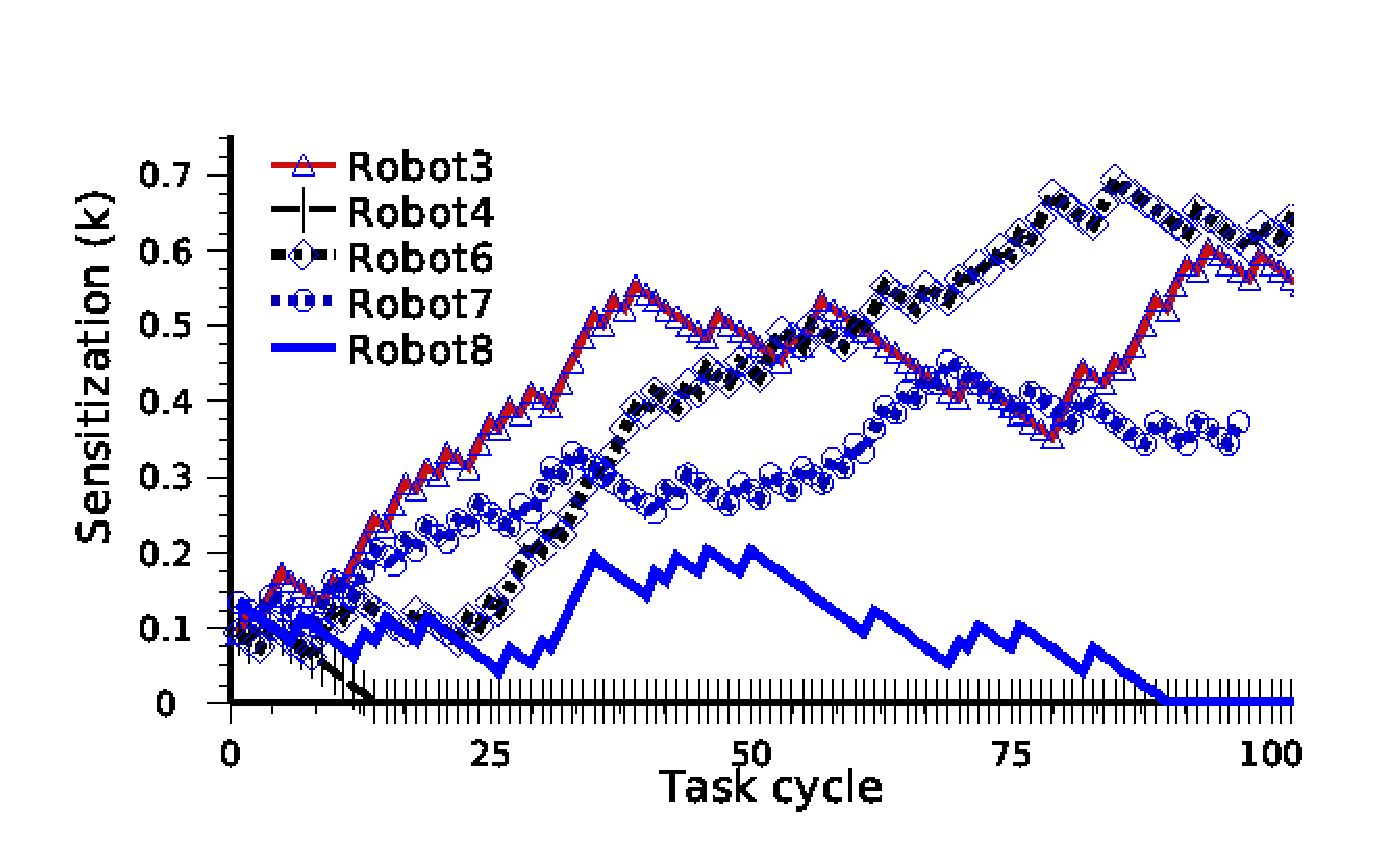
\includegraphics[width=0.7\textwidth, angle=0]{./TaskSpecialization-task3-10may-1.eps}
\caption{Task specialization on Task3 for a Series B experiment.}
\label{fig:k-single-task-SB} 
\end{figure}
%%
Fig. \ref{fig:k-single-task-SB} shows us the task specialization of five robots on Task3 in a particular run of Series B experiment. This shows us how some of the robots can specialize (learn) and de-specialize (forget) tasks over time.
%%-------------------------------------------------
\subsubsection{Robot motions}
We have aggregated the changes in translation motion of all robots over time. Let $u_{i,q}$ and $u_{i,q+1}$ be the translations of a robot $i$ in two consecutive steps. If the difference between these two translations be $\delta u_{i}$, we can find the sum of changes of translations of all robots in $(q+1)^{th}$ step using the following equation.
\begin{equation}
\Delta U_{q+1} = \sum_{i=1}^{N} \delta u_{i, q+1} 
\label{eqn:Delta-Tr}
\end{equation}
%%
\begin{figure*}
%\begin{minipage}[t]{0.5\linewidth}
\centering
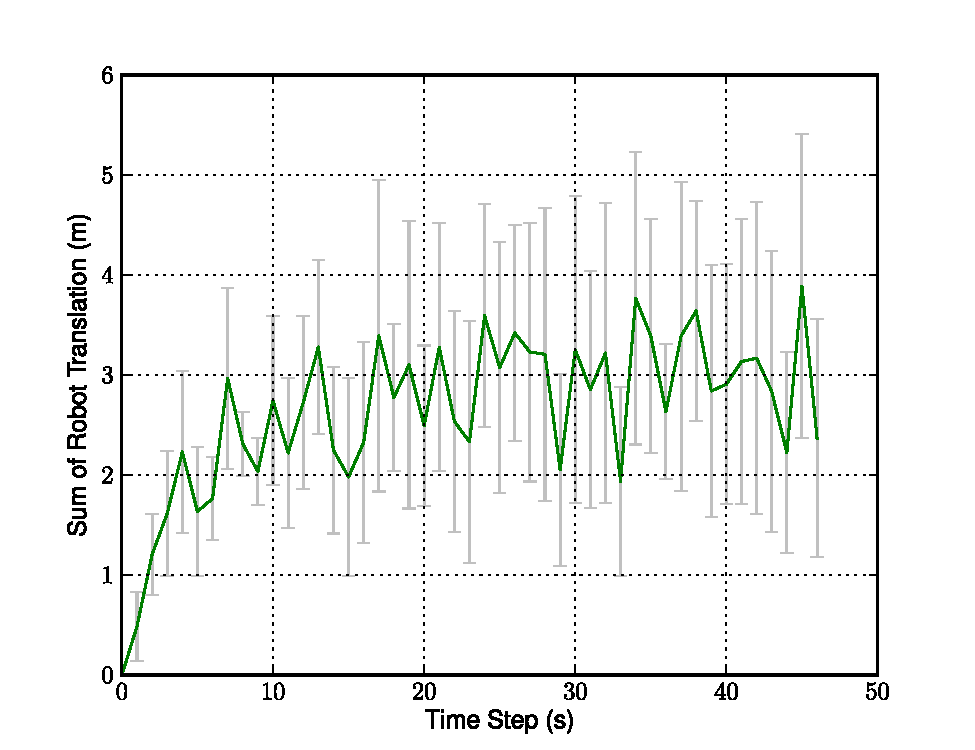
\includegraphics[width=0.7\textwidth]{./8robots-DeltaTranslationStat.eps}
\caption{\small Sum of the translations of robots in Series A experiments}
\label{fig:translation-stat-SA} % Give a unique label
%\end{minipage}
%\hspace{0.5cm}
%\begin{minipage}[t]{0.5\linewidth}
\centering
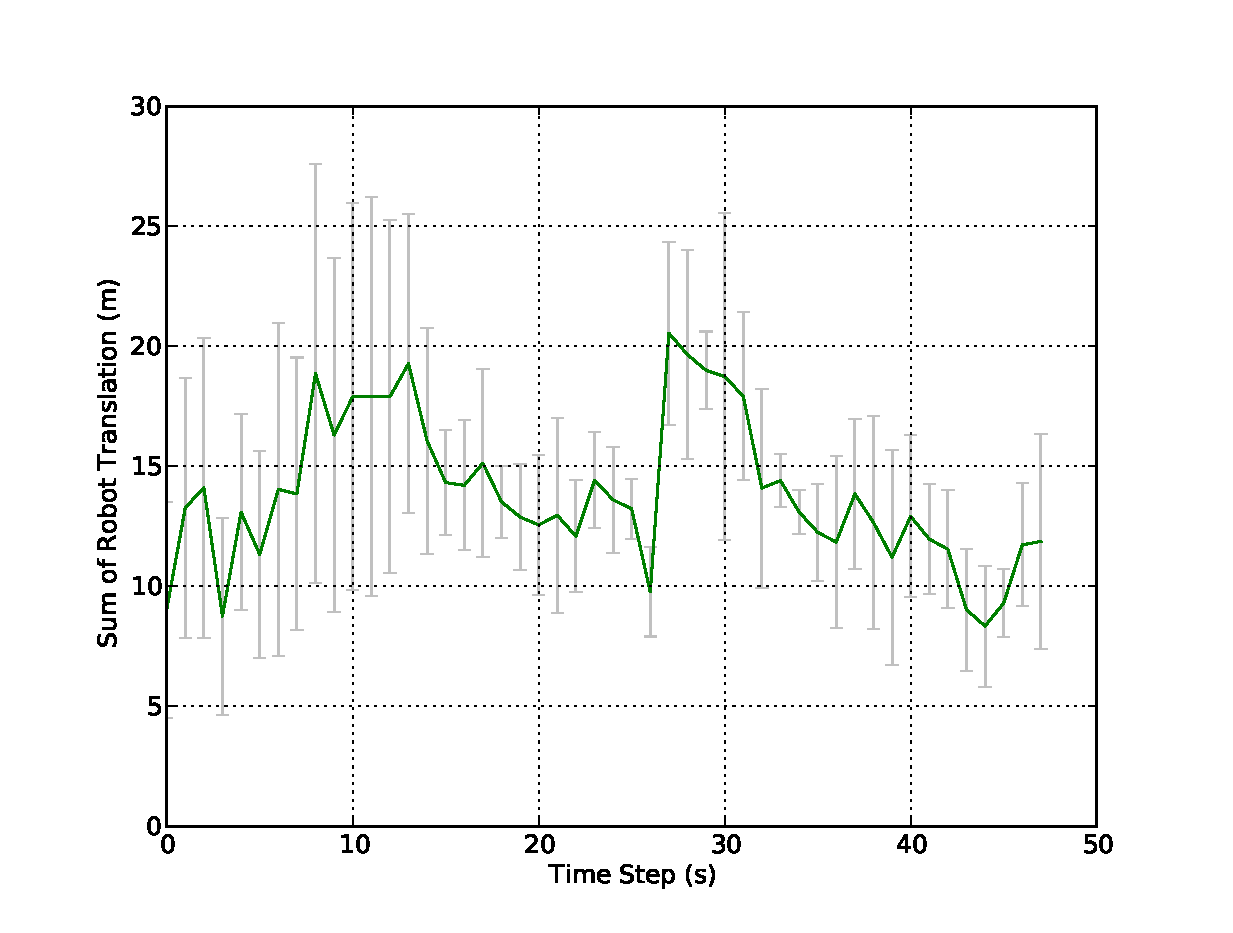
\includegraphics[width=0.7\textwidth]{./DeltaTranslationStat.eps}
\caption{\small Sum of the translations of robots in Series B experiments}
\label{fig:translation-stat-SB} % Give a unique label
%\end{minipage}
\end{figure*}
%%
The results from Series A and Series B experiments are plotted in Fig. \ref{fig:translation-stat-SA} and Fig. \ref{fig:translation-stat-SB}. In this plot we can see that robot translations also vary over varying task requirements of the manufacturing shop-floor scenario.
%%%-------------------------------------------------
\subsubsection{Communication load}
%%% Communication load %%%
\begin{figure}
%\begin{minipage}[t]{0.5\linewidth}
\centering
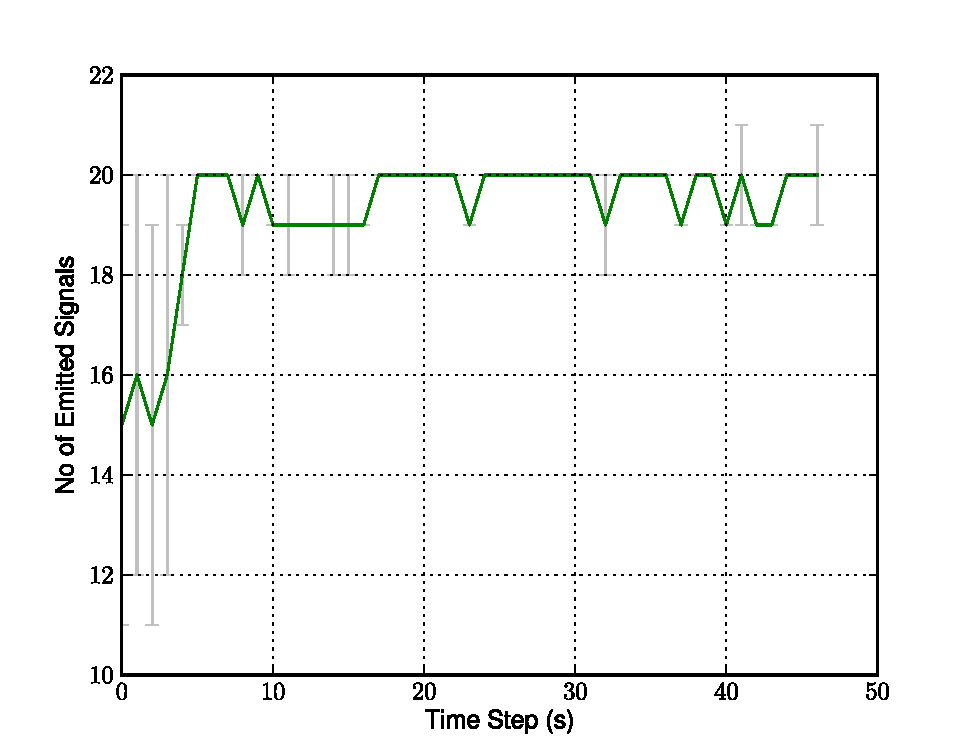
\includegraphics[width=0.7\textwidth]
{./8Robot-SignalingFreqStat.eps}
\caption{\small Frequency of \texttt{TaskInfo} signalling in Series A experiments}
\label{fig:signal-frequency-stat-SA} 
%\end{minipage}
%\hspace{0.5cm}
%\begin{minipage}[t]{0.5\linewidth}
\end{figure}
%%
\begin{figure}
\centering
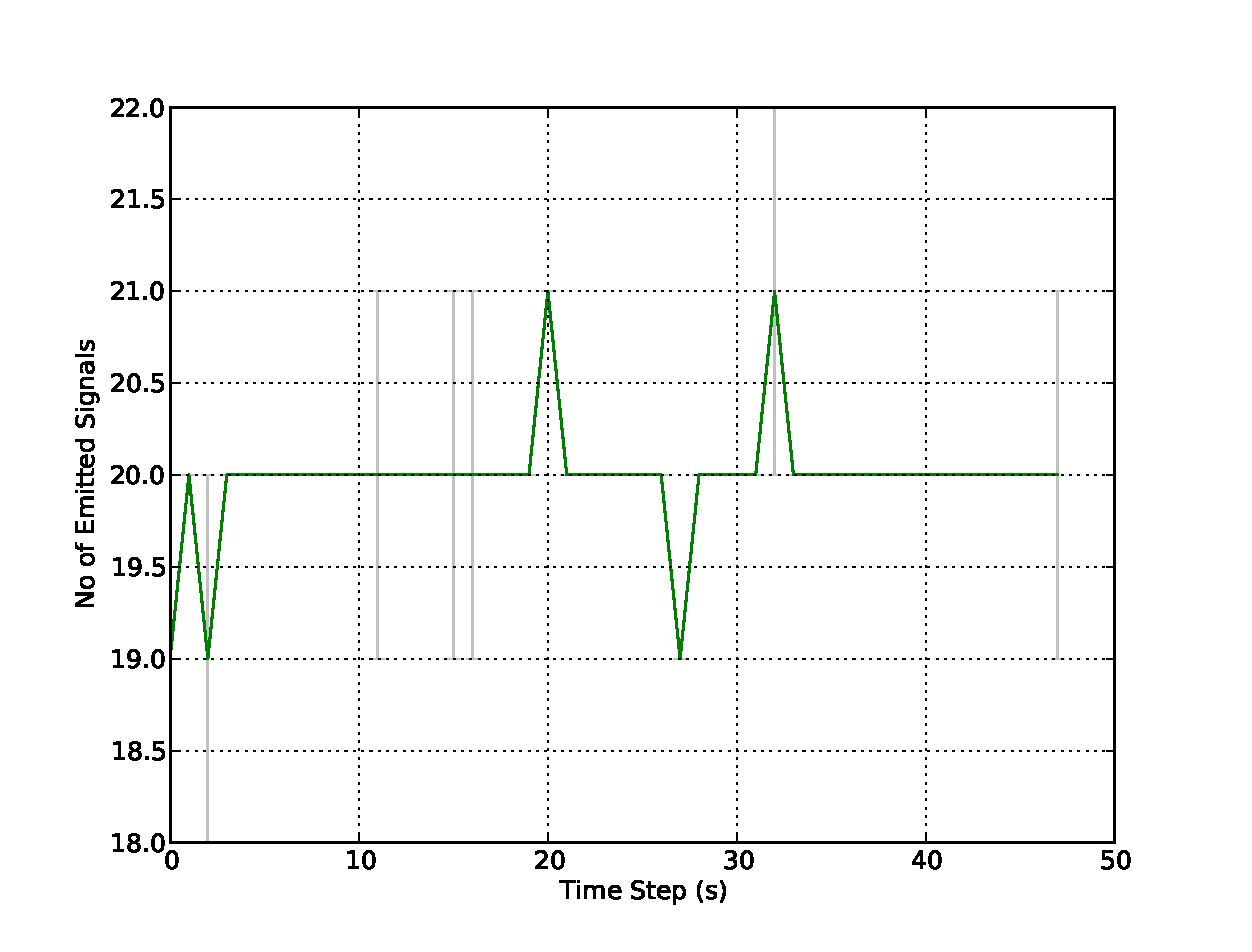
\includegraphics[width=0.7\textwidth]{./Global-SignalingFreqStat.eps}
\caption{\small Frequency of \texttt{TaskInfo} signalling in Series B experiments}
\label{fig:signal-frequency-stat-SB} 
%\end{minipage}
\end{figure}
%%
Fig. \ref{fig:signal-frequency-stat-SA}  and Fig. \ref{fig:signal-frequency-stat-SB}  show the number of received \texttt{TaskInfo} signals by each robot in Series A and Series B experiments. Since the duration of each time-step is 50s long and TPS emits signal in every 2.5s, there is an average of 20 signals in each time-step.
%--------------------------------------------------
\subsection{Discussions}
\label{afm:discuss}
%%-------------------------------------------------
Below we discusses our the major findings from the two types of MRTA experiments.
\subsubsection{Self-organized MRTA}
From our experimental results, we have noted several aspects of self-organized MRTA that exposes the power of AFM. As we have pointed out that self-organized MRTA, as observed in biological and human social systems, needs to satisfy several important characteristics, e.g. plasticity, task-specialization. In addition to satisfying those basic qualities, AFM has demonstrated many other aspects. Our self-organized robots, driven by AFM algorithms, effectively handle the dynamic work-load in our manufacturing shop-floor. They can dynamically support the need to work on currently demanding tasks, if there any. From the self-organized worker allocations under AFM, it is clear to us that although in larger system (Series B) the degree of variations of active-worker ratio can show us significantly unpredictable patterns, nevertheless the self-organized rules drive the robots to respond to the dynamic needs of the system. This means that AFM can sufficiently produce the plasticity of MRTA in order to meet the dynamic work-load of the system.
%%
\subsubsection{Learning and Forgetting}
From the individual and group-level task-specialization, we can see that robots can maintain both task-specialization and flexibility. In a self-organized system, it is very common that only a few individuals specialize on tasks and others generally do not. From two samples data sets, we can see that in particular runs of Series A and Series B experiments, task-sensitization values of  only 2-3 robots reach above the group-level average score. Thus in both types of experiments, robots exhibit similar task-specialization behaviours. From task-sensitization we can also see that a limited number of robots are specialized in tasks. Thus most of the other robots are flexible in selecting any tasks as their task-specializations do not bind them to particular tasks.
%%
\subsubsection{Concurrency and robustness}
As a consequence of fewer robots specializing in tasks, we can also see that robots can concurrently  consider different tasks without being biased to a particular task all the time. Our experiments also show us the robust MRTA as in case of  both high and low work-loads present in the system. This is evident from the manufacturing shop-floor task performance during production and maintenance cycles. For example,  in case of Series B experiments APMW was 65 seconds which corresponded  to pending work-load of 0.065 unit for a single robot. Thus, on an average, before the work-load exceeded by about 13 percent of initial work-load, robots were able to respond to  a task.
%%
\subsubsection{Communication load} 
In these experiments we used a centralized communication scheme as the source of attractive fields that serves the robot with necessary task-perception information. Although our robot-controllers software RCC was also co-located in the same host-PC, they can be distributed to several PCs or robot's on-board PCs.
%%
\subsubsection{Scaling-up}
We have observed the effect of scaling-up the robot team size. The system size of Series B is double than that of Series A in terms of robots, tasks and experiment arena. Keeping a fixed ratio of robot-to-task and task-to-arena we have intended to see the scaling effects in our experiments. Here we see that both systems can show sufficient self-organized MRTA, but task-performance of both systems varies significantly. For example, the value of production delay (APCD) in Series B is higher by 1.08. This means that performance  is decreased in Series B experiments despite having the resources in same proportion in both systems. This occurs partly due to the greater stochastic effects found in task-allocation in a larger system, e.g. presence of more tasks produce higher stochastic behaviours in robot's task selection.

Similarly we can see that in larger system robots have less chances to specialize on tasks, as the Series B experiments show us that the overall average task-specialization of the group $K^G_{avg}$ is lower by 0.10 and it lasts for lesser time (the difference of $Q^G_{avg}$  of both systems is 20 task-cycles). Thus, in a large group, robots are more likely to switch among tasks more frequently and this produces more translation motions which cost more energy (e.g. battery power) in task-performance.
%%====================================================
\section{Related Work}
\label{sec:rw}
%%--------------------------------------------------------------------
Traditionally MRTA solutions are classified into two broad categories: i) {\em explicit} and ii) {\em bio-inspired self-organized} task-allocation.  Explicit approach allocates task through explicit modelling of environment, tasks and robot capabilities. Some forms are: knowledge based \citep{Parker1998}, market based \citep{Dias+2006}, role/value based \citep{Chaimowicz2002}, control theoretic \citep{Belta+2004}. This approach is straight-forward to design, implement and analyse formally. But they are not suitable for large teams ($>$ 10)  and heavily dependent upon explicit global broadcast communication.  On the other hand self-organized approach is suitable for large teams since it has no explicit model and uses implicit/local communication. But this approach is difficult to design, implement, analyse and limited to one specific global task \citep{Gerkey+2004}. In an arbitrary event handling domain,  \cite{kalra+2007} reported that explicit task-allocation was more efficient when the required information could be captured accurately. The threshold-based approach offered similar quality of allocation at a fraction of cost in noisy environment. 
%%
\begin{table}
\label{table:so-afm}
\caption{Correspondence between the ingredients of self-organization and the requirements of self-organization under AFM}
\begin{center}
\begin{tabular}{|p{1.2in}|p{1.2in}|}
\hline  Ingredient of \protect\newline self-organization & Equivalent element under AFM \\ 
\hline Positive feedback &  Sensitization\\ 
\hline Negative feedback &  Forgetting\\ 
\hline Multiple interactions &  Continuous flow \protect\newline of information\\ 
\hline Amplification of fluctuations & -- \\ 
\hline  -- &  Concurrence\\ 
\hline 
\end{tabular} 
\end{center}
\end{table}

Task performance in self-organized approaches relies on the collective behaviours resulting from the local interactions of many simple and mostly homogeneous or interchangeable agents. Robots choose their tasks independently using general ingredients of self-organization such as: positive and negative feedback, multiple interactions among entities and their environment, and randomness or amplification of fluctuations \citep{Camazine+2001}. Table \ref{table:so-afm} compares the link between the so-called ingredients of self-organization and the corresponding requirements of self-organization in our model. Here we can see that the continuous flow of information can be approximately equivalent to the multiple interactions of the individuals of the group.

Among many variants of self-organized task-allocation mechanisms, the most common type is threshold-based task-allocation \citep{Bonabeau+1999}. In this approach, a robot's decision to select a particular task depends largely on its perception of a stimulus, e.g., the demand for a task to be performed, and its corresponding response threshold for that task. Under the deterministic response-threshold approach, each robot has an activation threshold for each task that needs to be performed. It continuously perceives or monitors the stimulus of all tasks that reflect the relative urgencies of tasks. When a particular task-stimulus exceeds a predefined threshold the robot starts working on that task, typically reducing the related stimuli. When the task-stimuli falls below the fixed threshold the robot abandons that task. This type of approach has been effectively applied in foraging \citep{Liu+2007,Krieger+2000} and aggregation \citep{Agassounon+2002}. 

The fixed response threshold can initially be same for all robots \citep{Jones+2000} or they can be different according robot capabilities or the configuration of the system \citep{Krieger+2000}. Adaptive response-threshold models change the thresholds over time. A robot's response threshold for a given task is often decreased as a result of the robot performing that task. This enables a robot to select that particular task more frequently or in other words specialise on that task \citep{Bonabeau+1999,Agassounon+2002}. Unlike the deterministic approach, where robots respond predictably, e.g., to the task stimulus that is the furthest above its threshold, probabilistic or stochastic approaches offer a selection process based-on a probability distribution over the tasks. In this case, all tasks commonly have at least a small, non-zero probability of being chosen. This random element typically prevents starvation of low stimulus tasks. 

The biological evidences of the existence of potential field between a task and an individual worker such as, a flower and a bee, a food source and an ant, inspired some researchers to conceptualize the assigning of artificial potential field between two manufacturing resources. For example, potential field is assumed between a machine that produce a material part and a worker robot or AGV that manipulates the raw materials and finished products. \cite{Ueda2006} conceptualized this potential field as the attractive and repulsive forces based on machine capabilities and product requirements. Task allocation is carried out based on the local matching between machine capabilities and product requirements. Each machine generates an attractive field based on its capabilities and each robot can sense and matches this attractive filed according to the requirements of a product. potential field is a function of distance between entities. Here, self-organization of manufacturing resources occurred by the process of matching the machine capabilities and requirements of moving robots. Through computer simulations and a prototype implementation of a line-less car chassis welding \cite{Ueda2006} found that this system was providing higher productivity and cost-effectiveness of manufacturing process where frequent reconfiguration of factory layout was a major requirement. 

Several other researchers did not express the above potential field for task allocation among manufacturing resources explicitly, rather they stressed on task selection of robots based on the task-capability broadcasts from the machines to the worker robots. In case of \cite{Lazinica+2007}, task capabilities are expressed as the required time to finish a task in a specific machine. They used assigned priority levels to accomplish the assembly of different kinds of products in the computer simulation of their bionic manufacturing system. 

In our work we have considered a manufacturing shop-floor scenario where robots are required to attend mock production and machine-maintenance jobs in different machines in an arena using their {\em homing} behaviours. Our study significantly differs from the above works since our generic framework of self-regulation considers, not only the spatial distances to tasks and their dynamic urgencies but also the learning and forgetting of agents about tasks. Moreover, unlike the above deterministic approaches, our approach uses a probabilistic method for task allocation.
%%%%%%%%%%%%%%%%%%%%%%%%%%%%%%%%%%%%%%%%%%%%%%%%%%%%%%%%%%%%%%%%
\section{Conclusions and Future works}
\label{sec:conc}
In this paper  an inter-disciplinary generic model of self-organized MRTA has been validated by incorporating it in a multi-robot system consists of 8 and 16 e-puck robots under a manufacturing shop-floor scenario. A centralized communication scheme has been incorporated to realize this model. Our model has been tested against a set of observables which include task-specialization, plasticity, task-performance and gross translations of robots.  Our experimental results suggest that under our centralized  communication scheme, these observables can indicate sufficient multi-robot task-allocation.

Our centralized communication scheme broadcasts attractive fields as information to all the robots from a central server. This is advantageous in terms of the ease of implementation and operation. But this has the disadvantage of being  a single point of load and a single point of failure. In future, we will explore local peer-to-peer communication models to spread attractive fields among a large multi-robot team.

In this study, we have kept the interaction among robots for task-completion under manufacturing shop-floor scenario as simple as possible. This is done mainly for minimizing the time and complexity of real-robotic implementation. This study can possibly be extended in co-operative task performance where different individuals with variety of task-skills need to interact with each other directly. For example, we can consider complex manufacturing shop-floor scenarios where the assembly operations of machine parts require coordination among multiple tasks. 

Our validation of AFM has been limited to a group of homogeneous robots that has initially same level of task-sensitization. Moreover no dynamic task has been introduced during the run-time of our experiments. Due to the stochastic task-allocation process, we always were able to see the  variation in task-urgencies. But AFM can be applied to a more challenging environment with suddenly appearing (and disappearing) dynamic tasks that can resemble to the real-world use-cases where any task can be pre-empted by other tasks. Moreover, some more research can be done in order to figure out how to optimize the initial experimental parameters, e.g. robots' task learning and forgetting rate. 

Finally, in terms of real-world implementation, we can consider to put AFM to solve many challenging industrial automation tasks. For example, AFM can be used to solve the automated material handing tasks in ware-houses and factories, or in real manufacturing tasks with suitable hardware modules. %In this way, our interdisciplinary model can help to overcome the existing challenges in the industry.
%%
%\bigskip
%\subsubsection*{Acknowledgements. } 
\begin{acknowledgements}
This research has been funded by the Engineering and Physical Sciences Research Council (EPSRC), UK, grant reference EP/E061915/1.
\end{acknowledgements}
%%
\begin{thebibliography}{22}
\providecommand{\natexlab}[1]{#1}
\providecommand{\url}[1]{{#1}}
\providecommand{\urlprefix}{URL }
\expandafter\ifx\csname urlstyle\endcsname\relax
  \providecommand{\doi}[1]{DOI~\discretionary{}{}{}#1}\else
  \providecommand{\doi}{DOI~\discretionary{}{}{}\begingroup
  \urlstyle{rm}\Url}\fi
\providecommand{\eprint}[2][]{\url{#2}}

\bibitem[{Agassounon and Martinoli(2002)}]{Agassounon+2002}
Agassounon W, Martinoli A (2002) {Efficiency and robustness of threshold-based
  distributed allocation algorithms in multi-agent systems}. In: Proceedings of
  the first international joint conference on Autonomous agents and multiagent
  systems: part 3, p 1097

\bibitem[{Arcaute et~al.(2008)Arcaute, Christensen, Sendova-Franks, Dahl,
  Espinosa, and Jensen}]{Arcaute+2008}
Arcaute E, Christensen K, Sendova-Franks A, Dahl T, Espinosa A, Jensen HJ
  (2008) Division of labour in ant colonies in terms of attractive fields. Ecol
  Complexity

\bibitem[{Belta and Kumar(2004)}]{Belta+2004}
Belta C, Kumar V (2004) {Abstraction and control for groups of robots}. IEEE
  Transactions on Robotics 20(5):865--875

\bibitem[{Bonabeau et~al.(1999)Bonabeau, Dorigo, and Theraulaz}]{Bonabeau+1999}
Bonabeau E, Dorigo M, Theraulaz G (1999) Swarm intelligence: from natural to
  artificial systems. Oxford University Press

\bibitem[{Camazine et~al.(2001)Camazine, Franks, Sneyd, Bonabeau, Deneubourg,
  and Theraula}]{Camazine+2001}
Camazine S, Franks N, Sneyd J, Bonabeau E, Deneubourg J, Theraula G (2001)
  Self-organization in biological systems. Princeton, N.J. : Princeton
  University Press

\bibitem[{Chaimowicz et~al.(2002)Chaimowicz, Campos, and
  Kumar}]{Chaimowicz2002}
Chaimowicz L, Campos MFM, Kumar V (2002) Dynamic role assignment for
  cooperative robots. Robotics and Automation, Proceedings ICRA'02 IEEE
  International Conference

\bibitem[{Dias et~al.(2006)Dias, Zlot, Kalra, and Stentz}]{Dias+2006}
Dias MB, Zlot RM, Kalra N, Stentz A (2006) Market-based multirobot
  coordination: A survey and analysis. Proceedings of the IEEE 94:1257--1270

\bibitem[{Gerkey and Mataric(2001)}]{Gerkey+2001}
Gerkey B, Mataric M (2001) {Principled communication for dynamic multi-robot
  task allocation}. Experimental Robotics VII pp 353--362

\bibitem[{Gerkey and Mataric(2004)}]{Gerkey+2004}
Gerkey BP, Mataric MJ (2004) A formal analysis and taxonomy of task allocation
  in multi-robot systems. The International Journal of Robotics Research 23:939

\bibitem[{Jones and Mataric(2003)}]{Jones+2000}
Jones C, Mataric M (2003) {Adaptive division of labor in large-scale minimalist
  multi-robot systems}. In: Proceedings of 2003 IEEE/RSJ International
  Conference on Intelligent Robots and Systems, 2003 (IROS 2003)

\bibitem[{Kalra and Martinoli(2007)}]{kalra+2007}
Kalra N, Martinoli A (2007) A comparative study of market-based and
  threshold-based task allocation. Distributed Autonomous Robotic Systems 7 pp
  91--101

\bibitem[{Krieger and Billeter(2000)}]{Krieger+2000}
Krieger M, Billeter J (2000) The call of duty: Self-organised task allocation
  in a population of up to twelve mobile robots. Robotics and Autonomous
  Systems 30(1-2):65--84

\bibitem[{Kube(1997)}]{Kube1997}
Kube CR (1997) Task modelling in collective robotics. Autonomous Robots
  4:53--72

\bibitem[{Lazinica and Katalinic(2007)}]{Lazinica+2007}
Lazinica A, Katalinic B (2007) Bionic assembly system: new concept of
  self-organising multirobot system. International Journal of Automation and
  Control 1(1):16--27

\bibitem[{Lerman et~al.(2006)Lerman, Jones, Galstyan, and
  Mataric}]{Lerman+2006}
Lerman K, Jones C, Galstyan A, Mataric MJ (2006) Analysis of dynamic task
  allocation in multi-robot systems. The International Journal of Robotics
  Research 25:225

\bibitem[{Liu et~al.(2007)Liu, Winfield, Sa, Chen, and Dou}]{Liu+2007}
Liu W, Winfield AFT, Sa J, Chen J, Dou L (2007) Towards energy optimization:
  Emergent task allocation in a swarm of foraging robots. Adaptive Behavior
  15(3):289--305

\bibitem[{Lochmatter et~al.(2008)Lochmatter, Roduit, Cianci, Correll, Jacot,
  and Martinoli}]{Lochmatter+2008}
Lochmatter T, Roduit P, Cianci C, Correll N, Jacot J, Martinoli A (2008)
  Swistrack-a flexible open source tracking software for multi-agent systems.
  In: Proc. of IEEE/RSJ International Conference on Intelligent Robots and
  Systems, 2008. IROS 2008, pp 4004--4010

\bibitem[{Parker(1998)}]{Parker1998}
Parker LE (1998) Alliance: an architecture for fault tolerant multirobot
  cooperation. Robotics and Automation, IEEE Transactions on 14:220--240

\bibitem[{Parker(2008)}]{Parker2008}
Parker LE (2008) Distributed intelligence: Overview of the field and its
  application in multi-robot systems. Journal of Physical Agents, special issue
  on multi-robot systems 2(2):5--14

\bibitem[{Pennington et~al.(2010)Pennington, Carlsson, and
  Larsson}]{Pennington+2010}
Pennington H, Carlsson A, Larsson A (2010) D-bus specification.
  \urlprefix\url{http://dbus.freedesktop.org/doc/dbus-specification.html}

\bibitem[{Sarker and Dahl(2010)}]{Sarker2010control}
Sarker M, Dahl T (2010) {Flexible Communication in Multi-robotic Control System
  Using HEAD: Hybrid Event-driven Architecture on D-Bus}. In: Proc. of the
  UKACC International Conference on Control 2010 (CONTROL 2010), Coventry, UK,
  pp 926--931

\bibitem[{Ueda(2007)}]{Ueda2006}
Ueda K (2007) Emergent synthesis approaches to biological manufacturing systems. Digital Enterprise Technology pp 25--34

\end{thebibliography}
% BibTeX users please use one of
%\bibliographystyle{spbasic} 
%\bibliographystyle{spmpsci}
%\bibliographystyle{splncs}
%\bibliographystyle{agsm}            
%\bibliography{Sarker_Dahl_ANTS2010_Special_issue} % name your BibTeX data base
\end{document}
